\documentclass[a4paper,11pt]{book}

%\documentclass[a4paper,twoside,11pt,titlepage]{book}
\usepackage{listings}
\usepackage[utf8]{inputenc}
\usepackage[spanish]{babel}


\usepackage{pgfgantt}
\usepackage{rotating}

\usepackage{algorithm}
\usepackage{algpseudocode}



%\usepackage[style=list, number=none]{glossary} %
%\usepackage{titlesec}
%\usepackage{pailatino}

\decimalpoint
\usepackage{dcolumn}
\newcolumntype{.}{D{.}{\esperiod}{-1}}
\makeatletter
\addto\shorthandsspanish{\let\esperiod\es@period@code}
\makeatother


%\usepackage[chapter]{algorithm}
\RequirePackage{verbatim}
%\RequirePackage[Glenn]{fncychap}
\usepackage{fancyhdr}
\usepackage{graphicx}
\usepackage{afterpage}

\usepackage{longtable}

\usepackage[pdfborder={000}]{hyperref} %referencia

% ********************************************************************
% Re-usable information
% ********************************************************************
%elimino \xspace
\newcommand{\myTitle}{Biblioteca de algoritmos para detección de anomalías.}
\newcommand{\mySubTitle}{Algoritmos basados en técnicas de proximidad.}
\newcommand{\myDegree}{Grado en Ingeniería Informática\xspace}
\newcommand{\myName}{Miguel Ángel López Robles }
\newcommand{\myProf}{Francisco Herrera Trigueros }
\newcommand{\myOtherProf}{Jacinto Carrasco Castillo }
%\newcommand{\mySupervisor}{Put name here\xspace}
\newcommand{\myFaculty}{Escuela Técnica Superior de Ingenierías Informática y de
Telecomunicación\xspace}
\newcommand{\myFacultyShort}{E.T.S. de Ingenierías Informática y de
Telecomunicación\xspace}
\newcommand{\myDepartment}{Departamento de Ciencias de la Computación
e Inteligencia Artificial}
\newcommand{\myUni}{\protect{Universidad de Granada}\xspace}
\newcommand{\myLocation}{Granada\xspace}
\newcommand{\myTime}{\today\xspace}
\newcommand{\myVersion}{Version 0.1\xspace}


\newenvironment{codigo}
 {\par\addvspace{\topsep}
  \centering
  \begin{minipage}{\linewidth}
  \hrule\kern2pt}
 {\par\kern2pt\hrule
  \end{minipage}
  \par\addvspace{\topsep}}

\algnewcommand\algorithmicforeach{\textbf{for each}}
\algdef{S}[FOR]{ForEach}[1]{\algorithmicforeach\ #1\ \algorithmicdo}

\hypersetup{
pdfauthor = {\myName (email (en) ugr (punto) es)},
pdftitle = {\myTitle},
pdfsubject = {},
pdfkeywords = {palabra_clave1, palabra_clave2, palabra_clave3, ...},
pdfcreator = {LaTeX con el paquete ....},
pdfproducer = {pdflatex}
}

%\hyphenation{}


%\usepackage{doxygen/doxygen}
%\usepackage{pdfpages}
\usepackage{url}
\usepackage{colortbl,longtable}
\usepackage[stable]{footmisc}


%\usepackage{index}

%\makeindex
%\usepackage[style=long, cols=2,border=plain,toc=true,number=none]{glossary}
% \makeglossary

% Definición de comandos que me son tiles:
%\renewcommand{\indexname}{Índice alfabético}
%\renewcommand{\glossaryname}{Glosario}

\pagestyle{fancy}
\fancyhf{}
\fancyhead[LO]{\leftmark}
\fancyhead[RE]{\rightmark}
\fancyhead[RO,LE]{\textbf{\thepage}}
\renewcommand{\chaptermark}[1]{\markboth{\textbf{#1}}{}}
\renewcommand{\sectionmark}[1]{\markright{\textbf{\thesection. #1}}}

\setlength{\headheight}{1.5\headheight}

\newcommand{\HRule}{\rule{\linewidth}{0.5mm}}
%Definimos los tipos teorema, ejemplo y definición podremos usar estos tipos
%simplemente poniendo \begin{teorema} \end{teorema} ...
\newtheorem{teorema}{Teorema}[chapter]
\newtheorem{ejemplo}{Ejemplo}[chapter]
\newtheorem{definicion}{Definición}[chapter]

\definecolor{gray97}{gray}{.97}
\definecolor{gray75}{gray}{.75}
\definecolor{gray45}{gray}{.45}
\definecolor{gray30}{gray}{.94}

\lstset{ frame=Ltb,
     framerule=0.5pt,
     aboveskip=0.5cm,
     framextopmargin=3pt,
     framexbottommargin=3pt,
     framexleftmargin=0.1cm,
     framesep=0pt,
     rulesep=.4pt,
     backgroundcolor=\color{gray97},
     rulesepcolor=\color{black},
     %
     stringstyle=\ttfamily,
     showstringspaces = false,
     basicstyle=\scriptsize\ttfamily,
     commentstyle=\color{gray45},
     keywordstyle=\bfseries,
     %
     numbers=left,
     numbersep=6pt,
     numberstyle=\tiny,
     numberfirstline = false,
     breaklines=true,
   }
 
% minimizar fragmentado de listados
\lstnewenvironment{listing}[1][]
   {\lstset{#1}\pagebreak[0]}{\pagebreak[0]}

\lstdefinestyle{CodigoC}
   {
	basicstyle=\scriptsize,
	frame=single,
	language=C,
	numbers=left
   }
\lstdefinestyle{CodigoC++}
   {
	basicstyle=\small,
	frame=single,
	backgroundcolor=\color{gray30},
	language=C++,
	numbers=left
   }

 
\lstdefinestyle{Consola}
   {basicstyle=\scriptsize\bf\ttfamily,
    backgroundcolor=\color{gray30},
    frame=single,
    numbers=none
   }


\newcommand{\bigrule}{\titlerule[0.5mm]}


%Para conseguir que en las páginas en blanco no ponga cabecerass
\makeatletter
\def\clearpage{%
  \ifvmode
    \ifnum \@dbltopnum =\m@ne
      \ifdim \pagetotal <\topskip
        \hbox{}
      \fi
    \fi
  \fi
  \newpage
  \thispagestyle{empty}
  \write\m@ne{}
  \vbox{}
  \penalty -\@Mi
}
\makeatother

\usepackage{pdfpages}
\begin{document}
\begin{titlepage}
 


 
\newlength{\centeroffset}
\setlength{\centeroffset}{-0.5\oddsidemargin}
\addtolength{\centeroffset}{0.5\evensidemargin}
\thispagestyle{empty}

\noindent\hspace*{\centeroffset}\begin{minipage}{\textwidth}

\centering

\includegraphics[width=0.9\textwidth]{imagenes/logo_ugr.jpg}\\[1.4cm]

\textsc{ \Large TRABAJO FIN DE GRADO\\[0.2cm]}
\textsc{ INGENIERÍA EN INFORMÁTICA}\\[1cm]
% Upper part of the page
% 
% Title
{\Huge\bfseries \myTitle \\
}
\noindent\rule[-1ex]{\textwidth}{3pt}\\[3.5ex]
{\large\bfseries \mySubTitle}
\end{minipage}

\vspace{2.5cm}
\noindent\hspace*{\centeroffset}\begin{minipage}{\textwidth}
\centering

\textbf{Autor}\\ \myName\\[2.5ex]
\textbf{Directores}\\ \myProf\\[2cm]


\includegraphics[width=0.3\textwidth]{imagenes/etsiit_logo.png}\\[0.1cm]
\textsc{Escuela Técnica Superior de Ingenierías Informática y de Telecomunicación}\\
\textsc{---}\\
Granada, 28 de mayo de 2019
\end{minipage}
%\addtolength{\textwidth}{\centeroffset}
%\vspace{\stretch{2}}
\end{titlepage}



\chapter*{}
%\thispagestyle{empty}
%\cleardoublepage

%\thispagestyle{empty}

\begin{titlepage}
 
 
\setlength{\centeroffset}{-0.5\oddsidemargin}
\addtolength{\centeroffset}{0.5\evensidemargin}
\thispagestyle{empty}

\noindent\hspace*{\centeroffset}\begin{minipage}{\textwidth}

\centering
%
\includegraphics[width=0.9\textwidth]{imagenes/logo_ugr.jpg}\\[1.4cm]

%\textsc{ \Large PROYECTO FIN DE CARRERA\\[0.2cm]}
%\textsc{ INGENIERÍA EN INFORMÁTICA}\\[1cm]
% Upper part of the page
% 

 \vspace{3.3cm}

%si el proyecto tiene logo poner aquí
%
\includegraphics{imagenes/logo.png} 
% \vspace{0.5cm}

% Title

{\Huge\bfseries \myTitle\\
}
\noindent\rule[-1ex]{\textwidth}{3pt}\\[3.5ex]
{\large\bfseries \mySubTitle\\[4cm]}
\end{minipage}

\vspace{2.5cm}
\noindent\hspace*{\centeroffset}\begin{minipage}{\textwidth}
\centering

\textbf{Autor}\\ \myName \\[2.5ex]
\textbf{Directores}\\
\myProf\\[2cm]
%Nombre Apellido1 Apellido2 (tutor2)}\\
%
\includegraphics[width=0.15\textwidth]{imagenes/tstc.png}\\[0.1cm]
%\textsc{Departamento de Teoría de la Señal, Telemática y Comunicaciones}\\
%\textsc{---}\\
%Granada, mes de 201
\end{minipage}
%\addtolength{\textwidth}{\centeroffset}
\vspace{\stretch{2}}

 
\end{titlepage}






\cleardoublepage
\thispagestyle{empty}

\begin{center}
{\large\bfseries \myTitle: \mySubTitle}\\
\end{center}
\begin{center}
\myName\\
\end{center}

%\vspace{0.7cm}
\noindent{\textbf{Palabras clave}: detección de anomalias, 
biblioteca python, aprendizaje no supervisado, clustering}\\

\vspace{0.7cm}
\noindent{\textbf{Resumen}}\\

En este trabajo se ha implementado una biblioteca en Python, para ofrecer
ayuda y resolución al problema de detección de anomalías. Para ello se han
implementado diversos algoritmos basados en la proximidad entre los distintos
ejemplos de datos. Se han implementado algoritmos de carácter más general y
tradicional, a la vez que se a buscado algoritmos innovadores y que profundizan 
más en los distintos inconvenientes que establece este reto. Con el fin de
analizar y comprobar la calidad de cada algoritmo, se ha desarrollado una 
experimentación con más de 20 conjuntos de datos. Con dicha experimentación,
buscaremos determinar las mejores condiciones para cada algoritmo.
\cleardoublepage


\thispagestyle{empty}


\begin{center}
{\large\bfseries 
Algorithm library for outlier detection: 
Algorithms based on proximity techniques}\\
\end{center}
\begin{center}
\myName\\
\end{center}

%\vspace{0.7cm}
\noindent{\textbf{Keywords}: outlier detection, Python library, unsupervised learning, 
}\\

\vspace{0.7cm}
\noindent{\textbf{Abstract}}\\

In this work, a Python library has been implemented, to offer help and resolution to the
anomaly detection problem. For this, diverse algorithms based on the proximity between the
different data examples have been implemented. we have implemented algorithms some classic
algorithms as well as some new algorithms that represent the state-of-the-art of the resolution
of the anomaly detetion problem. In order to analyze and
verify the quality of each algorithm, an experimentation with more than 20 data sets has been developed.
With this experimentation, we determine which are the best conditions for each algorithm.

\chapter*{}
\thispagestyle{empty}

\noindent\rule[-1ex]{\textwidth}{2pt}\\[4.5ex]

Yo, \textbf{Miguel Ángel López Robles}, alumno de la titulación Ingeniría Informática de la \textbf{Escuela Técnica Superior
de Ingenierías Informática y de Telecomunicación de la Universidad de Granada}, con DNI 76065425D, autorizo la
ubicación de la siguiente copia de mi Trabajo Fin de Grado en la biblioteca del centro para que pueda ser
consultada por las personas que lo deseen.

\vspace{6cm}

\noindent Fdo: Miguel Ángel López Robles

\vspace{2cm}

\begin{flushright}
Granada a 24 de junio de 2019 .
\end{flushright}


\chapter*{}
\thispagestyle{empty}

\noindent\rule[-1ex]{\textwidth}{2pt}\\[4.5ex]

D. \textbf{\myProf}, Profesor del Departamento de Ciencias de la Computación e Inteligencia Artificial  de la Universidad de Granada.

\vspace{0.5cm}

%D. \textbf{Nombre Apellido1 Apellido2 (tutor2)}, Profesor del Área de XXXX del Departamento YYYY de la Universidad de Granada.


\vspace{0.5cm}

\textbf{Informan:}

\vspace{0.5cm}

Que el presente trabajo, titulado \textit{\textbf{\myTitle, \mySubTitle}},
ha sido realizado bajo su supervisión por \textbf{\myName}, y autorizamos la defensa de dicho trabajo ante el tribunal
que corresponda.

\vspace{0.5cm}

Y para que conste, expiden y firman el presente informe en Granada a 24 de junio de 2019 .

\vspace{1cm}

\textbf{Los directores:}

\vspace{5cm}

\noindent \textbf{\myProf}% \ \ \ \ \ Nombre Apellido1 Apellido2 (tutor2)}

\chapter*{Agradecimientos}
\thispagestyle{empty}

       \vspace{1cm}



Muchas gracias a toda mi familia por el apoyo incondicional en todos estos años,
sin el cual no hubiera sido posible todos estos años de estudio. A mis profesores,
que tanto me han enseñado y que han ayudado a forjar la persona que soy. Por último
y más importante a Andrea que me apoyo cuando más lo necesitaba.

%\frontmatter
\tableofcontents
\listoffigures
%\listoftables
%
%\mainmatter
%\setlength{\parskip}{5pt}


\chapter{Introducción}


En la actualidad la extracción de conocimiento sobre datos está
adquiriendo cada vez más una mayor relevancia en el campo de la
ciencia de la computación y, con ello, una mayor aplicación en el
mundo industrial y empresarial. Este crecimiento se traduce en la
necesidad de investigación e innovación en las técnicas de minería
de datos.


En concreto, la detección de anomalías surge como un problema
específico, pero a la vez de gran relevancia, que consiste en la
identificación de aquellas instancias del conjunto de datos que,
debido a que se desvían del resto, se convierten en un caso con
un gran interés.

Un importante enfoque para la detección de anomalías es el basado
en la idea de proximidad, por el que consideraremos que una instancia
es una anomalía si es similar a las instancias que se encuentran
próximas \cite{aggarwalOutlierAnalysis2017}.  Se considerarán tanto técnicas basadas en
clustering, donde se identifica como instancias anómalas aquellas
que se sitúan en pequeños clústeres o se encuentran alejadas del
clúster al que se han asignado; las basadas en distancias y en técnicas
como el k-NN \cite{ishimtsevConformalKNNAnomaly2017}; y las técnicas basadas en densidad,
donde interviene el número de puntos existentes en una región local.

En este proyecto proponemos la realización de una biblioteca en Python
de métodos de detección de anomalías basados en proximidad, así como
la comparación de su eficacia en distintos ámbitos y la eficiencia de
estos métodos.



\section{¿Qué es una anomalía?}
Una anomalía es un punto de datos que es significativamente diferente
de los datos restantes. Hawkins definió [249] un valor atípico de la siguiente manera:



\textit{
 ``Una anomalía es una observación que se desvía tanto de las
otras observaciones como para despertar sospechas de que fue generado
por un mecanismo diferente"}


Como podemos ver este problema es realmente interesante y tiene un alto valor,
como nos menciona \textbf{Eugene Nathaniel Butler} \cite{quotationsEugeneNathanielButler}, estos casos especiales,
o diferentes pueden ser los más importantes.

\textit{
``Nunca tome el comentario de que usted es diferente como una condena,
podría ser un cumplido. Podría significar que posees cualidades únicas
que, como el más raro de los diamantes, es... único en su clase."}

En la minería de datos podemos encontrar diferentes términos para referirnos
a una anomalía como valor atípico, discordante,
desviaciones o datos fuera de lo normal. Cuando tomamos datos de una aplicación
podemos recibir información de uno o más procesos de generación,
lo cual puede reflejarse en la actividad del sistema y en las observaciones recopiladas.
Cuando el proceso de generación se comporta de manera inusual, resulta en la creación de anomalías.
Por lo tanto, un valor atípico a menudo contiene información muy útil sobre propiedades
anormales de los sistemas y entidades que afectan el proceso de generación de datos.
La detección de tales características inusuales proporciona información útil y específica de la aplicación.
La aplicación de la detección de anomalías puede aplicarse a numerosos campos como los siguientes:

\begin{itemize}
    \item \textbf{Sistemas de detección de intrusos.} En los sistemas informáticos, se recopilan diferentes
    tipos de datos como las llamadas del sistema operativo, el tráfico de la red u otras acciones de los usuarios.
    Estos datos pueden mostrar un comportamiento extraño debido a la actividad maliciosa. El reconocimiento de dicha
    actividad puede ser clave para evitar problemas mayores \cite{kumarAnomalyBasedNetworkIntrusion2019}
    \cite{jabezIntrusionDetectionSystem2015}.
    \item \textbf{Diagnóstico médico.} En la mayoría de aplicaciones médicas, los datos se recopilan de una variedad
    de dispositivos, como las imágenes por resonancia magnética (IRM), la tomografía por emisión de positrones (PET)
    o las series cronológicas de electrocardiogramas (ECG). Detectar patrones inusuales en tales datos, nos ayudará a
    detectar enfermedades
    \cite{vIdentificationOutliersMedical2014} \cite{gasparSystematicReviewOutliers2011}.
    \item \textbf{Fraude con tarjetas de crédito.} El fraude con tarjetas de crédito se ha vuelto un problema latente
    en nuestra sociedad, debido a la mayor facilidad con que la información confidencial, como el PIN de una tarjeta de crédito,
    puede verse comprometido. En la mayoría de casos, el uso no autorizado de una tarjeta de crédito puede mostrar diferentes patrones,
    como la compra desde ubicaciones particulares o transacciones muy grandes. Dichos patrones pueden usarse para detectar
    anomalías en los datos de transacciones y evitar dichos fraudes, determinando que operaciones son lícitas
    \cite{porwalCreditCardFraud2018} \cite{amrutad.pawarSurveyOutlierDetection2014}.
\end{itemize}

Como podemos ver en estas aplicaciones, los datos tienen un modelo conocido o normal, y las anomalías se reconocen como
desviaciones de este modelo normal. También podemos ver algunas aplicaciones, como la detección de intrusión o fraude,
donde los valores atípicos corresponden a secuencias de múltiples puntos de datos en lugar de puntos de datos individuales.
Por ejemplo, si pensamos en un fraude de tarjeta de crédito, puede ser detectado a través de una secuencia de acciones
inusuales. Este tipo de anomalías se conocen como colectivas y son a menudo el resultado de eventos inusuales que generan patrones
anómalos de actividad. En nuestro caso vamos a abordad algoritmos que busquen resolver problemas del mismo tipo que el diagnóstico
médico, es decir donde las anomalías no son secuencias de datos si no un ejemplo fuera de lo común.

\section{Aprendizaje no supervisado}
En nuestro caso los algoritmos estudiados abordan el problema desde el aprendizaje no supervisado, es decir, no disponemos de ejemplos,
previos, si no que los algoritmos deben ser válidos para cualquier entrada sin disponer de información adicional. Por tanto, en este escenario
no tenemos información de los datos ni conocemos el límite entre datos y error. Otra forma de afrontar este reto sería desde el aprendizaje
supervisado. Si se disponen de ejemplos y conjuntos de entrenamiento, podemos considerar las anomalías como una clase. Esto lo convierte
en un problema de clasificación donde podemos usar todas las herramientas que el matching learning nos ofrece, como puede ser las SVM y redes
neuronales. Esta tiene un requisito que en nuestro problema, convierte inviable esta opción.
Necesitamos un gran número de ejemplos y para tener un buen entrenamiento lo deseable sería tener también ejemplos de la clase de anomalías.
En nuestro escenario, este requisito es difícil de cumplir, ya que lo normal es disponer de pocos ejemplos de anomalías, además de que queremos
una solución que sea capaza de afrontar cualquier nueva anomalía que surge y no solo las conocidas.

En definitiva, estamos en un problema de aprendizaje no supervisado, donde a partir de unos datos de entrada sin etiquetar, debemos extraer
que ejemplos se consideran anomalías.




\section{¿Existe solución?}

El problema de detección de anomalías no es un problema con una solución trivial, la cual podemos obtener con simples procesos.
Como hemos visto se trata de una pregunta compleja y no es fácil determinar que se define como algo típico o normal y
algo atípico o diferente. Para remarcar este hecho vamos a plantear un pequeño ejemplo de datos:

\begin{figure}[h]
    \center{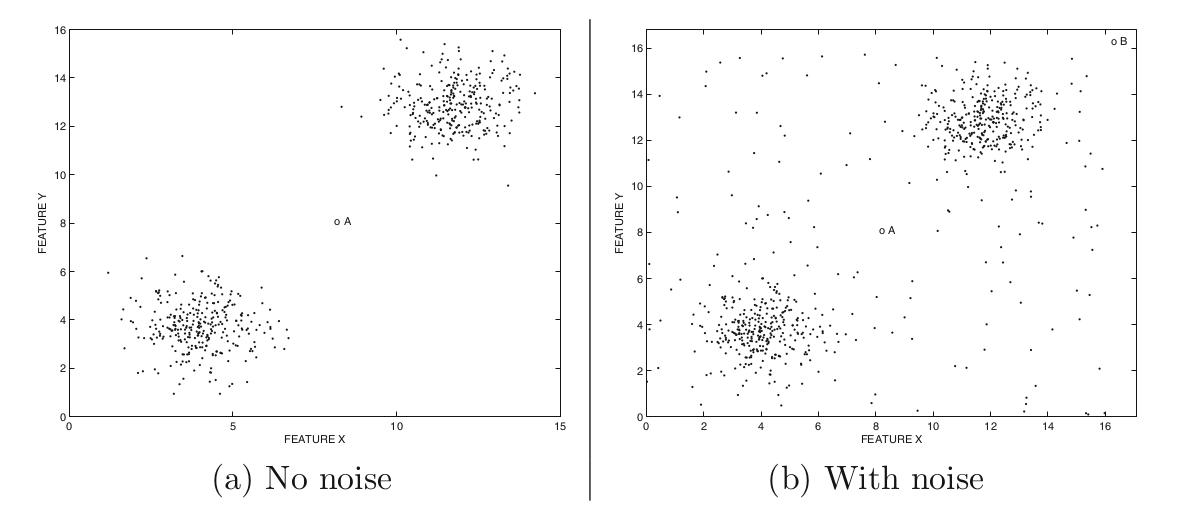
\includegraphics[width=\textwidth]
    {imagenes/ejemplo_basico.jpeg}}
    \caption{\label{fig:my-label} Ejemplo de datos con ruido}
\end{figure}

Como podemos ver en el caso a), la respuesta a si el punto A es una anomalía o no es más fácil. Pero en el caso b) la respuesta
deja de ser tan obvia y empezamos a plantearnos hasta qué punto podemos determinar si un punto es anomalía o no. En datos reales
el problema aumenta, ya que tendremos más dimensiones, cada una con su ruido y una medición podrá desviarse en unas dimensiones y 
en otras seguir el modelo actual. La respuesta ha si hay solución al problema ya no es tan clara. Por tanto, vamos a ver que dos
respuestas se han ofrecido como respuesta a nuestro problema:

\begin{itemize}
    \item \textbf{\textit{Score} de anomalía.} La mayoría de los algoritmos de detección de anomalías responden con una puntuación que cuantifica
    el nivel de ``anomalía" de cada punto de datos. Esta puntuación también se puede utilizar para ordenar los puntos de datos en
    orden para conocer cuáles pueden ser considerados "más" extraños. Esta es una forma muy general cuantificar y resolver el problema,
    que mantiene la información proporcionada por un algoritmo, pero no ofrece una respuesta clara o concisa sobre qué puntos son
    anomalías y cuáles no.
    \item \textbf{Etiqueta binaria.} En este tipo de salida obtenemos una etiqueta binaria por cada punto, indicándonos si se trata de una
    anomalía o no. Existen algunos algoritmos capaces de dar esta respuesta tan precisa, lo normal es usar la puntuación de anomalía. Como
    el resultado que finalmente queremos es una respuesta binaria, lo típico es trasformar las puntuaciones en etiquetas binarias. Para ello,
    normalmente se establecen umbrales en las puntuaciones y este determina puntos que son anomalías. Cuando marcamos un punto como anomalía,
    también estamos perdiendo información del grado de anomalía.
\end{itemize}

En definitiva, podemos decir que estamos enfrentando un problema complicado, cuya decisión de cuando constituye una desviación importante 
para que se considere anomalía no es trivial. A pesar de ello, existen multitud de perspectivas y distintos enfoques para la solución.
En nuestro caso vamos a usar tecnicas basadas en proximidad las cuales explicaremos más adelante.


\section{Motivación}

Este proyecto surge debido a la necesidad de tener una biblioteca de software con algoritmos capaces de afrontar diferentes situaciones de
detección de anomalías. Además, se ha realizado en Python, un lenguaje de programación en alza y muy usado para problemas relacionados con
la computación y la inteligencia artificial. Existe una biblioteca  también
enfocada a la resolución del problema de detección de anomalías\cite{zhaoPyODPythonToolbox2019}, pero este implementa
algoritmos más generalistas y de todos los tipos de enfoque, mientras que en 
nuestro caso queremos enfocarnos y profundizar en el estudio de los algoritmos 
basados en proximidad y aquellos que no son tan conocidos, pero pueden ofrecer un nuevo enfoque y buenos resultados.

La biblioteca se llama \textbf{PyDBOD Python Distances Based Outlier Detector}. Podemos encontrar los repositorios para 
instalar la biblioteca en los repositorios de GitHub \cite{Miki97TFGOutlierDetectionHttps} y en el repositorio de 
PyPI \cite{PyDBODDistancesBased}.
%

\chapter{Especificacion de requisitos}
\section{Requistos funcionales}
Nuestro proyecto pretende desarrollar una biblioteca competitiva y de 
gran utilidad. Para ello vamos a necesitar cumplir los siguientes requisitos:

\begin{itemize}
    \item \textbf{Alta velocidad de procesamiento.} Debemos tener en cuenta
    que estamos en un campo donde si queremos tener una aplicación real de
    nuestra biblioteca, esta debe ser rápida y dar una respuesta en un tiempo
    razonablemente pequeño. El reto viene dado porque en nuestra área suele
    trabajarse con grandes volúmenes de datos, lo que supone que si no realizamos
    los procedimientos de manera eficiente, nuestra biblioteca puede demorarse más
    tiempo del deseado.

    \item \textbf{Estandarización Sklearn.} La biblioteca Sklearn \cite{APIReferenceScikitlearn} 
    se ha establecido como un estándar en Python en cuanto a algoritmos y métodos
    relacionados con el matching learning. Por tanto, si queremos que nuestra biblioteca
    pueda llegar al mayor número de usuarios y sea de un uso fácil e intuitivo, deberemos
    seguir el estándar de clase que se establece en Sklearn.

    \item \textbf{Respuesta clara.} Si realizamos un pequeño vistazo a los algoritmos
    más conocidos, podemos observar que la salida de cada algoritmo ofrece su propia
    puntuación o score. Por tanto, para hacer nuestra biblioteca más funcional se
    realizará una estandarización de los resultados de cada algoritmo, transformando 
    la salida en una probabilidad y permitiendo la comparación entre diferentes algoritmos.

    \item \textbf{Seguridad.} Si queremos que nuestra biblioteca sea referente y realmente
    útil, necesitamos la seguridad de que los resultados que nos ofrecen son los correctos
    y no exista duda de si nuestra biblioteca puede tener un comportamiento erróneo. Para ello
    será un requisito muy importante la realización de una gran cantidad de pruebas, con el fin 
    de ofrecer el producto más fiable.

    \item \textbf{Experimentación con datos reales.} Un requisito de nuestra biblioteca será
    demostrar que funciona para cualquier situación que se pueda presentar y para cualquier
    conjunto de datos reales. Por tanto, es necesario una experimentación con un gran número
    de conjuntos de datos reales que demuestren el buen comportamiento de nuestra biblioteca
    ante cualquier problema de la vida cotidiana.

\end{itemize}

\section{Objetivos}
En primer lugar, vamos a definir los objetivos que se busca alcanzar en este 
proyecto y sobre los cuales se a desarrollado el trabajo realizado.
\begin{itemize}
    \item \textbf{Revisión de la bibliografía existente.} En primer lugar
    se pretende explorar los algoritmos y propuestas ya publicadas, además de
    lectura de libros especializados en la materia. Esto nos permite
    adquirir un conocimiento profundo en la materia y un
    mejor desarrollo y entendimiento de los algoritmos implementados.
    Además, nos aportará una base de algoritmos para su posible implementación.

    \item \textbf{Estudio de cada algoritmo y diseño.} El segundo objetivo es un 
    estudio en profundidad de cada algoritmo para conocer los detalles de
    implementación. Se debe realizar un patrón de diseño para generar
    estructuras generales y reutilizables para todos ellos.

    \item \textbf{Implementación y prueba.} El tercer objetivo será
    realizar una implementación de cada algoritmo, basándose en la
    bibliografía y la realización de pruebas para confirmar el correcto
    funcionamiento de estos. Para ello se comprobará su correcto funcionamiento
    tanto en datos sintéticos como en datos reales.

    \item \textbf{Comparación y análisis.} El último objetivo es la
    realización de una comparación entre los algoritmos implementados y 
    analizar el comportamiento, las ventajas y desventajas que cada uno
    de estos. Para así determinar cuáles serán los casos más atractivos para
    la utilización de cada algoritmo. Se probará con una gran
    batería de conjuntos de datos y con los resultados se extraerán conclusiones.
\end{itemize}




%
\chapter{Planificación}

\section{Planificación temporal}
El proyecto al cual nos enfrentamos tiene una dimensión considerable y
como hemos visto en los requisitos tenemos varios pasos complejos que
completar. Por tanto, la planificación debe ser fundamental. Cierto
es que el proceso de investigación está presente en todas las etapas,
pero en el siguiente diagrama veremos cómo se ha planificado el tiempo
para el desarrollo del proyecto

\begin{figure}[h]
\begin{ganttchart}[
    canvas/.append style={fill=none, draw=black!5, line width=.75pt},
    vgrid={*1{draw=black!5, line width=.75pt}},
    today=20,
    today label font=\scriptsize\scshape,
    title/.style={draw=none, fill=none},
    title label font=\scshape\footnotesize,
    title label node/.append style={below=7pt},
    include title in canvas=false,
    bar/.append style={draw=none, fill=black!63}
    ]{1}{20}


    \gantttitle{Sep}{2}
    \gantttitle{Oct}{2}
    \gantttitle{Nov}{2}
    \gantttitle{Dic}{2}
    \gantttitle{Ene}{2}
    \gantttitle{Feb}{2}
    \gantttitle{Mar}{2}
    \gantttitle{Abr}{2}
    \gantttitle{May}{2}
    \gantttitle{Jun}{2}
    \gantttitle{Jul}{2}\\

    \ganttbar{Investigación}{1}{6} \\
    \ganttbar{Análisis}{4}{8} \\
    \ganttbar{Diseño}{6}{8} \\
    \ganttbar{Implementación}{7}{18} \\
    \ganttbar{Pruebas}{11}{18} \\
    \ganttbar{Experimentación}{16}{20} \\
    \ganttbar{Memoria}{16}{20}

\end{ganttchart}
\caption{Planificación del proyecto}
\label{fig:gantt}
\end{figure}
En este diagrama de Gannt podemos ver que la planificación
era bastante clara. La primera fase era un proceso de investigación
y adquisición de una base de conocimientos que permitiera una comprensión
de los conceptos necesarios para el desarrollo del proyecto. Este proceso
conlleva un trabajo de inmersión en el campo a través de la lectura de libros
y artículos. El principal libro usado como referencia ha sido \cite{aggarwalOutlierAnalysis2017}.

A continuación, una etapa más de análisis y diseño de los algoritmos a implementar.
En esta etapa ya poseíamos una base de conocimientos fuertes para afrontar las especificaciones
de cada algoritmo. En esta etapa se analiza y se profundiza en los componentes
y desarrollo de cada algoritmo de nuestra biblioteca
Por último, tenemos la etapa de implementación, pruebas y experimentación, que 
en parte se han ido desarrollando en paralelo. En primer lugar, si existe una fase
de implementación del esquema general que siguen todos nuestros algoritmos y de la
base de partida. Después, en la implementación de cada algoritmo se prefirió probar
el funcionamiento tras la implementación de este. 

Como podemos ver existe un alto solapamiento entre las distintas etapas. Esto
se debe a que no se ha desarrollado con una metodología típicamente en cascada,
sino que se ha usado una metodología iterativa donde se iban realizando las 
fases de análisis, implementación y prueba de cada algoritmo hasta confirmar
su correcto funcionamiento. Una vez que se tenía un algoritmo listo se pasaba al
siguiente. De este modo podíamos profundizar mejor en la investigación y en los 
conceptos de cada algoritmo.

Por último, mencionar la etapa de desarrollo de la memoria donde se ha realizando
un trabajo de recopilación y de exposición de todo el trabajo que se ha realizado
durante este periodo de trabajo.


\section{Material necesario}
Para la implementación de este proyecto ha sido necesario un ordenador para el desarrollo.
En mi caso he utilizado mi ordenador personal, un Asus X550VX con un microprocesador de
Intel i5-6300HQ con cuatro núcleos físicos y 8 GB de RAM. Como podemos ver es un ordenador
no excesivamente potente y realmente con cualquier ordenador con un sistema Unix y un procesador
medianamente potente puede realizarse sin problema el desarrollo. Si debemos mencionar
que en cuanto a la memoria si han sido estrictamente necesarios los 8GB 
ya que manejamos grandes cantidades de datos y en algunos casos se ha alcanzado un uso de 
memoria de 7GB

También ha sido necesario una conexión a internet, recurso indispensable para acceder a la
documentación y paper de los algoritmos implementados. Además de proporcionar información
adicional ya sea en temas teóricos o de implementación. Este material es de fácil acceso y
en nuestro caso gratuito en la red de la universidad.




%
\chapter{Análisis de algoritmos}\label{cap:Analisis}

\section{Introducción}
Para el estudio de las técnicas basadas en proximidad, vamos a usar como
fuente principal de estudio el libro de Charu C. Aggarwal
\cite{aggarwalOutlierAnalysis2017}.

En primer lugar, vamos a analizar los conceptos básicos de las técnicas basadas
en proximidad. Estas técnicas definen un punto de datos como un valor 
atípico cuando su localidad (o proximidad) está poblada escasamente.
Existen varias formas de definir la proximidad de un punto de datos.
Estas definiciones son sutilmente diferentes entre sí, pero son lo suficientemente
similares como para agruparlas y realizar un tratamiento unificado 
dentro de un solo tipo. Las formas más comunes de definir la proximidad 
para la detección de anomalías son las siguientes:


\begin{itemize}
    \item \textbf{Basado en cluster.} La no pertenencia de un punto de 
    datos a cualquiera de los grupos, su distancia a otros grupos,
    el tamaño del grupo más cercano o una combinación de estos factores
    se utilizan para cuantificar la puntuación final de la anomalía.
    El problema de clustering tiene una relación complementaria
    con el problema de detección de valores atípicos, en el que los 
    puntos pertenecen a grupos o deben considerarse valores atípicos.
    \item \textbf{Basados en distancias.} La distancia de un punto de 
    datos a su k-vecino más cercano (u otra variante) se utiliza para 
    definir la proximidad. Los puntos de datos con grandes distancias 
    a sus k-vecinos más cercanos, se definen como valores atípicos. 
    Los algoritmos basados en la distancia generalmente realizan el 
    análisis con una granularidad mucho más detallada que los otros dos 
    métodos. Por otro lado, esta mayor granularidad a menudo tiene un 
    costo computacional significativo.
    \item \textbf{Basados en densidad.} La cantidad de otros puntos 
    dentro de una región local específica (una cuadrícula o 
    región basada en la distancia) de un punto de datos, 
    se utiliza para definir la densidad local. Estos valores de 
    densidad local se pueden convertir en la puntuación final. 
    También se pueden usar otros métodos basados en kernel o métodos 
    estadísticos para la estimación de la densidad. La principal diferencia 
    entre el clustering y los métodos basados en la densidad es que los 
    métodos de agrupación en clústeres dividen los puntos de datos, 
    mientras que los métodos basados en la densidad dividen el espacio 
    de datos.

\end{itemize}

No podemos negar que todas estas técnicas están estrechamente 
relacionadas porque se basan en alguna noción de proximidad (o similitud).
La principal diferencia está en el nivel de detalle con el cual se 
estima la proximidad. Es obvio que cada forma diferente de definir la 
proximidad y, por tanto, que es una anomalía, conlleva ciertas ventajas
y desventajas. En muchos casos, es difícil diferenciar en cuál de las
definiciones estamos trabajando ya que es muy usual usar más de un concepto
a la vez. Es por ello que también queda justificado su agrupación para un análisis conjunto.

Como ya hemos anunciado antes, una diferencia importante entre los 
métodos basados en distancias y los otros dos tipos, radica en el
nivel de granularidad en el que se realiza el análisis. Tanto en los 
métodos basados en clustering, como en densidad, los datos quedan 
agrupados antes del análisis y el cálculo de puntuación de anomalía.
Esta agrupación se realiza ya sea mediante la partición de los puntos
o del espacio. Cada punto del conjunto de datos se compara con las 
distribuciones en estos datos pre-agrupados para el análisis. Por
otro lado, en los métodos basados en distancias, la distancia del
k-vecino más cercano a los puntos de datos originales (o una variante 
similar) se calcula como la puntuación de anomalía. Por lo tanto, el 
análisis en los métodos del vecino más cercano se realiza a un nivel de 
granularidad más detallada que los métodos de agrupamiento. Dicho de otra manera
se analizan todos los puntos. Esta mayor granularidad conlleva una desventaja,
estos métodos proporcionan diferentes compensaciones entre la eficacia y la 
eficiencia para conjuntos de datos de diferentes tamaños. Los métodos en los
que calculamos el vecino más cercano pueden tener una complejidad $O(N^{2})$ para
calcular todas las distancias del vecino k más cercano para un conjunto de
datos de tamaño N. Es fácil de ver de dónde surge dicha
complejidad, ya que para cada punto deberemos de calcular la distancia con
el resto de puntos. Esta complejidad se puede reducir o acelerar si 
usamos alguna técnica de indexación o poda.

Pero el uso de estas técnicas no será algo trivial que nos solucione todos
nuestros problemas, las técnicas de indexación y poda generalmente 
funcionan bien solo en algunas configuraciones restringidas, como los 
conjuntos de datos de baja dimensionalidad. Además, la poda no está diseñada
para el problema que nos ocupa ya que puede ser altamente interesante tener
la puntuación final de todos los puntos, aunque no se considere anomalía. Por
ellos la poda solo podrá usarse en aquellas configuraciones en las que la
respuesta sea una etiqueta binaria que indica si un punto es anomalía.
al contrario de lo que esto nos podría hacer pensar, las técnicas 
del k-vecino más cercano o más conocidas como k-nn, son técnicas
con una alta popularidad y su uso es muy frecuente para diversas aplicaciones.
Esto se debe a que tales métodos a menudo son capaces de proporcionar un
análisis más detallado y preciso. Este hecho se amplifica en conjuntos de 
datos pequeños donde el agrupamiento o el análisis de densidad no es posible
o los resultados que ofrece son complicados. En definitiva, la elección de 
un modelo, definición o técnica, depende de la naturaleza de los datos y
su tamaño.

Las técnicas basadas en la proximidad de los datos, están diseñadas naturalmente
para detectar tanto el ruido como las anomalías. A pesar de ello existen 
métodos que se adecuan más para cada tarea. Por ejemplo, la definición
de una baja pertenencia de un punto a un grupo de datos, está diseñada
naturalmente para la detección de ruido. Mientras que, por otro lado 
una alta desviación o escasez de densidad o altas distancias pueden 
detectar mejor las anomalías. A pesar de ello los métodos basados en la 
pertenencia tienen también popularidad ya que son muy intuitivos y 
se dispone de una fácil explicación a la puntuación de una anomalía.
De hecho, varios métodos se basan en este tipo de definiciones, ya que 
por su simplicidad, se pueden generalizar fácilmente a casi todos los 
tipos de datos, tanto datos de series temporales, como datos de secuencia
o datos de gráficos.

Ahora vamos a analizar y explicar más detalladamente cada uno de los subgrupos
que hemos expuesto. Como ya hemos comentado anteriormente, aunque exista
un concepto principal en algunos algoritmos, la realidad es que muchos 
pueden interpretarse desde varias perspectivas y es difícil su clasificación
en un tipo u otro. A pesar de ello todas siguen siendo técnicas basadas 
en proximidad.


\section{Métodos basados en clustering}
Como ya comentamos anteriormente existe una fuerte conexión entre la detección
de anomalías y el clustering. Si vemos el problema de la detección de anomalías
desde este nuevo enfoque y con una visión simplista, podemos determinar que cada
punto puede ser miembro de un clúster o ser una anomalía. Aquellos puntos que
no se agrupen dentro de un clúster se pueden definir entonces como anomalía.
En el clustering, el objetivo principal es dividir los puntos en subconjuntos
densos. Por otro lado, en la detección de anomalías el objetivo es identificar
los puntos que no encajan fácilmente o de forma natural en estos subconjuntos
densos. De hecho, los algoritmos de clustering reportan valores atípicos como 
un producto secundario de su análisis.

Parece que hemos encontrado una solución fácil y buena a nuestro problema,
pero, sin embargo, es importante entender que usar solo la relación
complementaria de la pertenencia a los grupos para definir los
valores atípicos da como resultado el descubrimiento no solo anomalías si no
también del ruido. Esto se debe a que la no pertenencia de un punto a ningún
grupo de datos es una razón bastante directa para medir el nivel de
desviación de un punto de datos de los patrones normales.  Por ejemplo, 
normalmente un conjunto de puntos no suele estar muy concentrado en un único
punto, por tanto, un punto de datos que se encuentra en la periferia
de un grupo grande es muy diferente de uno que está completamente 
aislado de todos los otros grupos. Además, todos los puntos de datos
en grupos muy pequeños a veces también pueden considerarse anomalías. 
En definitiva, cuando se utiliza la agrupación en clústeres para la 
detección de anomalías, se utiliza un enfoque más matizado (que el de 
la no pertenencia a un grupo) para calcular las puntuaciones de los 
valores atípicos.


Podemos definir una definición simple para realizar una puntuación de anomalías
utilizando las distancias de los puntos de los puntos de datos a los centroides
generados al agrupar en clúster. Específicamente, la distancia de un punto
al centroide del grupo más cercano se puede usar como una buena característica
para la puntuación de valor atípico de un punto de datos. Dado que los grupos
pueden tener diferentes formas y orientaciones, una excelente medida de la
distancia que se debe utilizar es la distancia de \textit{Mahalanobis}, que escala los
valores de distancia según las variaciones locales del grupo, a lo largo de las
direcciones de la correlación. 

Vamos a ver cómo podemos aplicar la distancia \textit{Mahalanobis}. En primer
lugar, consideramos un conjunto de datos que contiene $k$ clústeres. Supongamos
que el grupo $rth$ en el espacio de $d$ dimensiones tiene un vector fila $d$-dimensiones
denotado por $\overline{\mu_r}$ que contiene la media de cada atributo. Por
otro lado disponemos de una matriz de covarianzas de dimensiones $d$ x $d$
definida como $\Sigma_r$. La entrada $(i,j)$ de esta matriz nos proporciona
la covarianza local entre las dimensiones $i$ y $j$ en el clúster. Con esto podemos
definir el cuadrado de la distancia \textit{Mahalanobis} entre un punto 
definido como vector-fila $\overline{X}$ con la siguiente expresión:

\begin{center}
    $MB(\overline{X}, \overline{\mu_r}, \Sigma_r)^2 = (\overline{X} - \overline{\mu_r})
    \Sigma_r^{-1} (\overline{X} - \overline{\mu_r})^T$
\end{center}
Después de que los puntos de datos se hayan calificado con la distancia
local de Mahalanobis, cualquier método se puede aplicar
como detector de anomalías para convertir estas puntuaciones en etiquetas binarias.

El efecto de la distancia de Mahalanobis es proporcionar
una normalización estadística basada en las características de un punto
de datos particular. Incluso aunque las distancias pequeñas a lo largo de las 
direcciones en las que se producen las variaciones del grupo son pequeñas
pueden ser estadísticamente significativas dentro de esa localidad de datos.
De manera análoga, las grandes distancias a lo largo de las direcciones
en las variaciones del grupo que son grandes pueden no ser,
estadísticamente significativas dentro de esa localidad de datos.
Dicho enfoque producirá resultados más refinados que un uso global
de la distancia Euclidia, porque se adapta mejor a la localidad de
datos en cuestión.

Para remarcar las propiedades y ventajas que nos ofrece el uso de la distancia
Mahalanobis vamos a plantear el ejemplo planteado en \cite{aggarwalOutlierAnalysis2017}:
\begin{figure}[h]
    \center{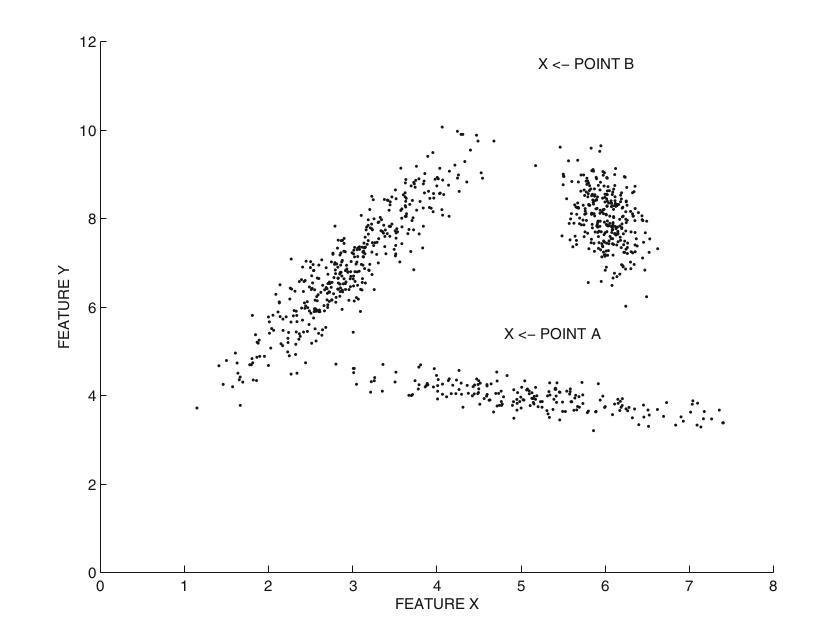
\includegraphics[width=\textwidth]
    {imagenes/distancia_mahalanobis.jpeg}}
    \caption{\label{fig:distance_maha} Ejemplo uso de la distancia Mahalanobis}
\end{figure}

Como podemos ver, en este ejemplo el punto A debería ser considerado una
anomalía con mayor facilidad que el punto B. Esto se debe a que el punto 
A no sigue ningún patrón y es algo claramente fuera de lo normal. Sin embargo
el punto B a pesar de estar alejado del clúster, puede verse como un punto
perteneciente al clúster ya que sigue el patrón, aunque se aleje más. Si aplicamos
la distancia Euclidia, el punto B está más lejos de los centroides que el
punto A. Por lo que el punto B obtendría una puntuación mayor que A. Sin 
embargo, si usamos la distancia Mahalanobis solventamos estos inconvenientes.


Además de los criterios basados en la distancia, es común usar el número
de puntos pertenecientes al conjunto como un componente de la puntuación
de valor atípico. Por ejemplo, el logaritmo negativo de la fracción de
puntos en el grupo más cercano se puede utilizar como un componente de
la puntuación de anomalía. Podemos crear dos vectores de puntuaciones
de N-dimensiones basados en los criterios de distancia y cardinalidad,
normalizar cada uno y luego agregarlos.

También debemos mencionar que los métodos basados en clustering tienen una alta
variabilidad de predicción ya que estos dependen de la elección del modelo especifico,
la inicialización aleatoria o la configuración de parámetros. Todos estos 
factores influyen en los resultados finales. Para ello será aconsejable realizar
varias mediciones y usar la media.

Como conclusión final de este tipo de métodos vamos a mencionar las ventajas
y desventajas que estos ofrecen. Una de las principales ventajas es que existen
algoritmos de clustering relativamente rápidos y que no alcanzan la complejidad
cuadrática de los algoritmos basados en distancias, como veíamos anteriormente.
La principal desventaja de los métodos de clustering es que no siempre proporcionan
la información al nivel de detalle requerido. La granularidad de los métodos de análisis
de valores atípicos es generalmente mejor cuando se utilizan cálculos de
distancia directamente con los puntos de datos originales, en lugar de con
respecto a representantes agregados, como los centroides de los clústeres.



\section{Métodos basados en distancias}
Los métodos basados en distancias son una clase popular de algoritmos 
de detección de anomalías en una amplia variedad de tipos de datos.
Estos definen puntuaciones de los valores atípicos en función de las 
distancias del vecino más cercano. El ejemplo más simple es el caso en 
el que la distancia del vecino más cercano $k$ de un punto se
usa como su puntuación. Como podemos ver es un método simple y por ello,
a menudo es fácil generalizar esta técnica a otros tipos de datos como 
datos categóricos, datos de texto, datos de series de tiempo y datos de 
secuencia.

Los métodos basados en la distancia funcionan con la suposición natural 
de que las distancias del vecino $k$ más cercano de las anomalías
son mucho mayores que las de los puntos de datos normales.


Como ya hemos mencionado con anterioridad, las técnicas basadas en distancias
nos proporcionan una gran granularidad de análisis en comparación con los métodos
de clustering. Esta propiedad puede permitir una capacidad más refinada 
para distinguir entre ruido y anomalías. Para analizar este hecho vamos a
recordar el ejemplo de la Introducción donde como veíamos no era fácil
distinguir entre ruido y anomalías.

\begin{figure}[h]
    \center{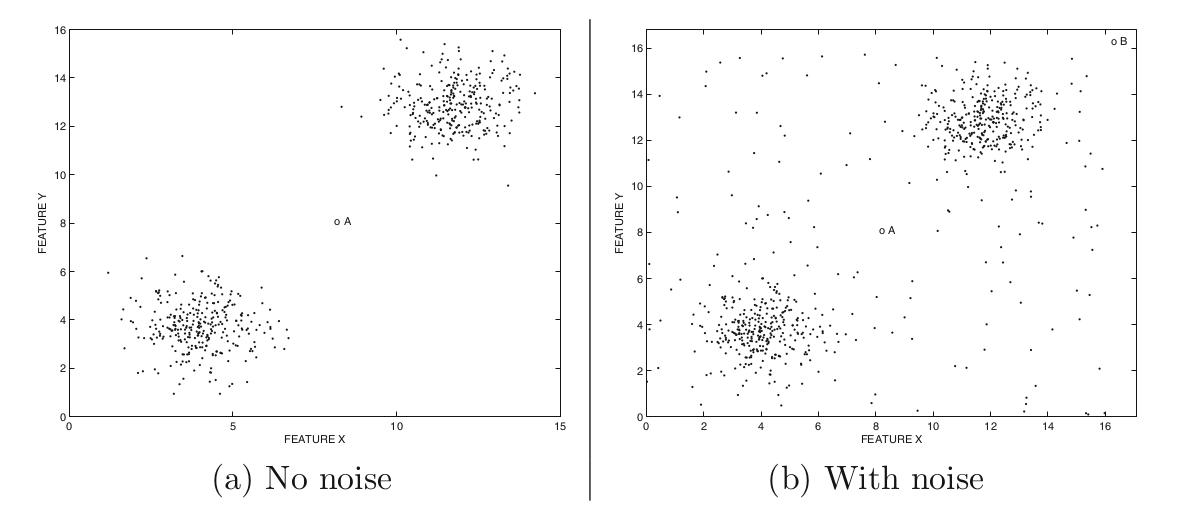
\includegraphics[width=\textwidth]
    {imagenes/ejemplo_basico.jpeg}}
    \caption{\label{fig:my-label} Ejemplo de datos con ruido}
\end{figure}

Como podemos ver en la figura, un algoritmo de clustering no sería capaz de 
distinguir entre ruido y anomalías. Esto se debe a que la distancia al centroide 
de clúster más cercano para el punto de datos $A$ seguirá siendo la misma en 
ambos casos. Por otro lado, un algoritmo vecino más cercano k (k-nn) distinguirá entre 
estas situaciones porque los puntos de datos ruidosos se incluirán entre 
las evaluaciones de distancia. Por otro lado, el enfoque de clustering no 
podrá distinguir estas situaciones con un resultado tan bueno porque los 
centroides de cada clúster son relativamente insensibles al ruido en 
los datos. Por supuesto, también es posible modificar métodos basados en
clústeres para incluir los efectos del ruido. En esos casos, los dos
enfoques convergen y pasan a ser enfoque muy similares. Esto se debe a 
que como hemos mencionado anteriormente, aunque los consideremos tipos distintos,
en realidad los dos tipos de métodos están estrechamente relacionados.
 

La funcionalidad de este tipo de métodos es muy alta, también pueden 
identificar grupos aislados de anomalías estrechamente relacionados.
Por ejemplo, para identificar un grupo pequeño que contiene $k_0$
puntos de datos, es necesario usar un valor de $k \geq k_0$ en el algoritmo
de vecino más cercano. Aunque dichas anomalías también se pueden identificar
mediante métodos de clustering al establecer un umbral en la cantidad de
puntos en cada clúster, a veces estos puntos pueden agruparse en clúster 
y sesgar los centroides correspondientes. Esto como podemos imaginar puede 
afectar el proceso de puntuación atípica de manera muy negativa.


El resultado más general de los métodos basados en la distancia es en 
forma de score. Si necesitamos la puntuación de todos los puntos será
necesario el cálculo de las distancias relativas a cada punto y, por tanto,
necesitamos una complejidad de $O(N^{2})$. En el caso de que necesitemos una
respuesta binaria, si se identifica un punto como anomalía es posible la 
aplicación de varios tipos de poda y estructuras de indexación, con lo que
conseguiremos una alta ganancia de velocidad.


\subsection{Métodos basados en distancias para puntuación}
La puntuación de anomalía basada en la distancia de un punto
se fundamenta en la distancia del vecino más cercano $k$ . 
Hay dos variaciones simples de este mecanismo de puntuación conocidos como
el k-nearest neighbor exacto y el k-nearest neighbor promedio:




\begin{itemize}
    \item \textbf{k-nn exacto.} Se usa como puntuación la distancia al
    $k$ vecino más lejano donde $k$ es un parámetro que debemos establecer.
    Debemos tener en cuenta que no podemos usar la distancia del punto
    así mismo ya que esto podría afectar a los resultados. El problema
    de este enfoque es la elección correcta del valor para $k$. Un buen
    resultado dependerá de nuestra elección. En problemas no supervisados,
    como la detección de valores atípicos, a menudo no hay manera de 
    ajustar los parámetros con métodos como la validación cruzada,
    ya que tales métodos requieren un conocimiento extra de la información.
    \item \textbf{k-nn con media.} En este caso se realiza el cálculo del
    $k$ vecino más cercano. En este caso en lugar de usar solo la distancia
    de este vecino se usa el promedio de los $k$ vecinos más cercanos, es decir,
    aquellos que su distancia es menor a la del $k$ vecino.
    de datos. En este caso el parámetro $k$ no influye tan fuerte como en el caso
    anterior. Por tanto si conocemos el valor correcto de $k$, el k-nn exacto
    nos proporciona mejores resultados, pero si no podemos mitigar este error
    usando el promedio de las distancias.
    \item \textbf{k-nn con media armónica.} Igual que en el caso anterior
    solo que usamos la media armónica para calcular la puntuación. Debemos
    tener cuidado de eliminar los valores repetidos. Este tipo de media siempre
    este dominada por distancias pequeñas y por tanto si usamos un valor alto
    para k, incluso en el caso de usar $ k = N$, conseguiremos una alta robustez.
    
\end{itemize}

\subsection{Métodos basados en distancias para etiquetas binarias}
En esta variedad de los métodos basados en distancias se obtiene una salida
de etiqueta binaria, que determina si un punto es una anomalía o no. Este
enfoque limita el número de aplicaciones en el cual podemos hacer uso de 
esta técnica, pero tiene una gran ventaja. En el caso anterior hablábamos de 
que era totalmente necesario una complejidad de $O(N^2)$, en este caso con
el uso de etiquetas binarias podemos aplicar ciertas técnicas de poda.


En este esquema solo los scores más altos serán considerados como anomalías 
y no debemos preocuparnos por la puntuación específica de cada punto.
para conseguir este objetivo, la técnica que principalmente se usa, es determinar
un umbral de puntuación $\beta$ a partir del cual, los puntos que lo superen se consideran
anomalías. También podemos verlo como establecer un umbral de la distancia mínima para 
ser considerado anomalía.


Ambos enfoques son en esencia idénticos y debemos de remarcar que conllevan 
añadir un nuevo parámetro $\beta$ que se usará para determinar el umbral. 
Este hecho aumenta la complejidad de nuestro problema y es que es necesario
una correcta elección de dicho parámetro y será fundamental en los resultados.


Por tanto, el proceso se compondrá de un cálculo de todas las distancias y una
posterior clasificación para aplicar el umbral. Esto como podemos imaginar sigue
siendo un cálculo bastante costoso. Para obtener una mejora será necesario
realizar una poda. 


Existen varías técnicas como la poda basada en celdas donde se divide el espacio
en celdas. Para no entrar en detalles la idea básica será evitar el cálculo
repetitivo de otros puntos en la misma celda ya que los resultados serán muy similares.
Este algoritmo comienza a complicarse ya que ahora además se debe de ajustar 
el tamaño de dichas celdas.


Existen más técnicas de poda, con procedimientos más complejos como puede ser la 
poda basada en índices o la poda basada en muestreo. Todas estas técnicas son
interesantes, aunque en nuestro caso no son relevantes ya que nos centramos en técnicas
que aportan como resultado la puntuación final de anomalía.


\subsection{Ventajas y desventajas}
Los métodos basados en la distancia tienen una serie de ventajas 
sobre las técnicas basadas en clustering, debido a la granularidad 
más detallada del análisis. Por ejemplo, los algoritmos basados en la 
distancia pueden distinguir entre ruido y anomalías mucho mejor que los 
basados en técnicas de clustering. Además, los métodos basados en la
distancia también pueden encontrar grupos aislados de valores atípicos
al igual que los métodos de clustering. Sin embargo, los métodos de 
clustering tienen la ventaja de que
pueden proporcionar información sobre las distribuciones locales 
de puntos para definir distancias. También existen casos como el que veíamos
en la figura \ref{fig:distance_maha}, donde la estructura del clúster local se
puede utilizar para definir una distancia de Mahalanobis localmente 
sensible, que es mucho más efectiva en este caso, que una aplicación ciega de
la distancia Euclidia. También es posible la combinación y realización de
un enfoque basado en distancias que use la distancia Mahalanabis.

Aunque los métodos basados en la densidad que se explican más adelante
incorporan algunos conceptos de localidad, no pueden proporcionar el 
nivel detallado de información local que una combinación efectiva de 
un enfoque basado en clustering y distancia puede proporcionar. En esta
tendencia existen multitud de investigaciones, las cuales buscan agrupar
las ventajas que proporcionan cada tipo de algoritmos. Por un lado, la eficiencia
que aportan los métodos basados en clustering y por otro lado la granularidad
y los buenos resultados que ofrecen los métodos basados en distancias.

 




\section{Métodos basados en densidad}

Los métodos basados en la densidad utilizan la cantidad de puntos 
en regiones específicas del espacio para definir valores atípicos. 
Están muy estrechamente relacionados con el clustering y los métodos 
basados en la distancia. En realidad, algunos de estos algoritmos 
pueden considerarse más fácilmente como clustering o basados en la 
distancia, según cómo se presenten. Esto es porque la idea de distancias,
clustering y la densidad están estrechamente relacionadas y son dependientes
entre sí. Esta relación la veremos más clara cuando expliquemos los algoritmos
implementados, ya que, aunque la mayoría se pueden considerar de densidad, pueden
considerarse también basados en distancias o clustering, simplemente viendo 
los métodos desde otro enfoque.


Para comprender mejor el enfoque basado en densidad y la capacidad de detección
de estos métodos basados en localidad, vamos a ver un ejemplo que se muestra en
la siguiente figura del libro \cite{aggarwalOutlierAnalysis2017}:

\begin{figure}[h]
    \center{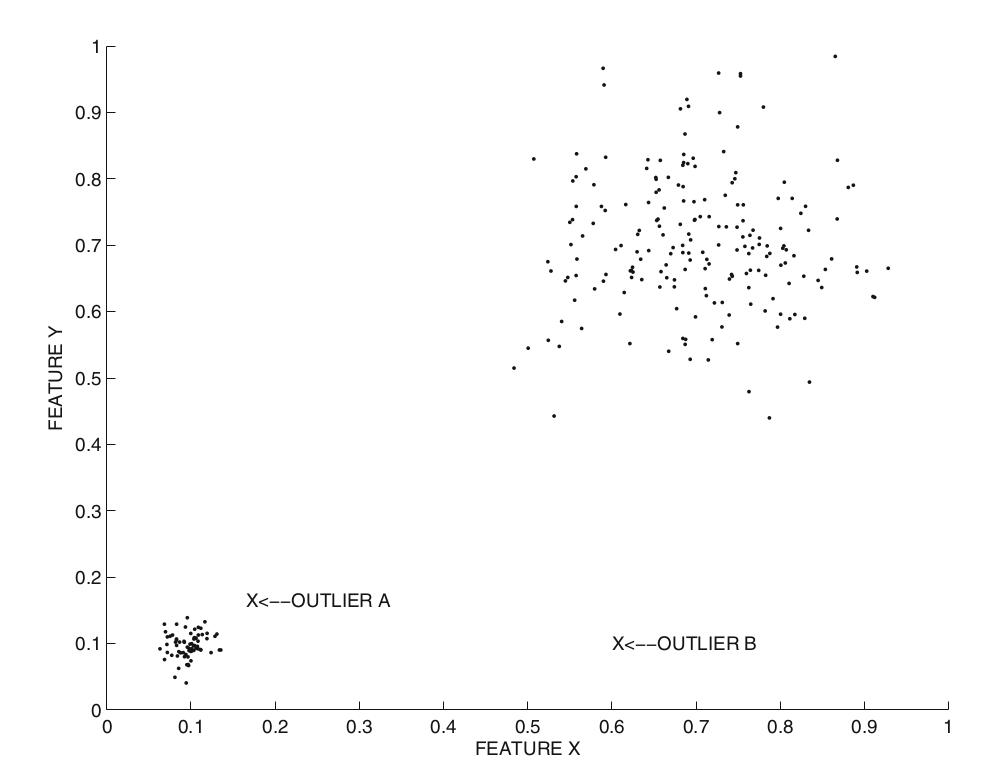
\includegraphics[width=\textwidth]
    {imagenes/ejemplo-densidad.jpeg}}
    \caption{\label{fig:densidad} Ejemplo detección por densidad}
\end{figure}

Esta figura contiene dos anomalías etiquetadas con A y B.Además, la figura 
contiene dos grupos, uno de los cuales es mucho más disperso que el otro.
Es evidente que los algoritmos basados en la distancia no pueden descubrir la
anomalía A, a menos que el algoritmo utilice un umbral de distancia muy pequeño.
El uso de este umbral para la distancia tan pequeño conlleva que muchos puntos
del grupo disperso también sean considerados anomalías, llevando a un resultado 
totalmente erróneo. Esto también significa que la clasificación devuelta por un
algoritmo basado en la distancia es incorrecta cuando hay heterogeneidad 
significativa en las distribuciones locales de los datos. Sin embargo, que mide la 
densidad de cada punto, podemos determinar que A y B son anomalías sin necesidad 
de asignar una alta puntuación al grupo de puntos disperso ya que estos detectarán
una mayor densidad a su alrededor. Por ello estos algoritmos son muy interesantes.


Gran parte del trabajo en clustering basado en densidad generalmente 
se ha centrado en cuestiones de densidad de datos variable en lugar de la forma 
y orientación variable de los grupos, como comentábamos en el análisis de la figura
\ref{fig:distance_maha}


Otros métodos combinan los algoritmos de \textbf{k-nn} con variaciones locales de 
densidad. El más claro ejemplo de aplicación de estos conceptos es \textbf{LOF} 
\cite{breunigLOFIdentifyingDensitybased2000}, algoritmo que explicaremos más adelante
y que hemos implementado en nuestra biblioteca.
%
\chapter{Diseño}
Para el desarrollo de nuestro paquete de algoritmos hemos usado una
estructura de clases siguiendo el patrón de sklearn \cite{APIReferenceScikitlearn}.
Para ello se ha diseñado una clase abstracta que sirve como patrón 
de diseño para todas las clases que implementen un algoritmo.
Ya que estamos en un problema de aprendizaje no supervisado el método
principal para el uso de cada algoritmo será \texttt{fit predit(datos)} .
Vamos a ver primero un esquema de nuestra clase abstracta
De este modo facilitamos el uso de la biblioteca a todos los usuarios
haciendo fácil, homogéneo e intuitivo su uso.
 
\begin{figure}[h]
    \center{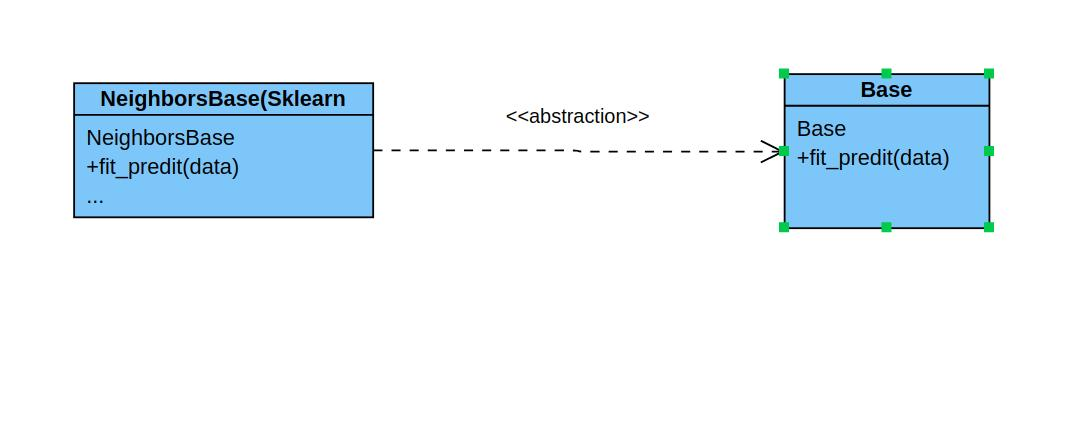
\includegraphics[width=\textwidth]
    {imagenes/base-abstraccion.jpeg}}
    \caption{\label{fig:base-abstraccion} Abstracción de la clase general sklearn}
\end{figure}

A partir de nuestra clase \texttt{Base} el resto de algoritmos se
implementaran en una clase que herede de esta. De este modo aseguramos
la homogenización dentro de los distintos algoritmos de la biblioteca.
Si algún algoritmo necesita un método auxiliar podría declararse, pero el 
método de uso siempre será a través de \texttt{fit predit(datos)}.

Para cada algoritmo podremos declarar 
los parámetros necesarios en la creación de un objeto de la clase. Por 
tanto los parámetros de ajuste para cada algoritmo serán parámetros del 
constructor de cada clase.

Para ver más claramente la estructura final de nuestro paquete, veamos
el diagrama de clases:
\begin{figure}[H]
    \center{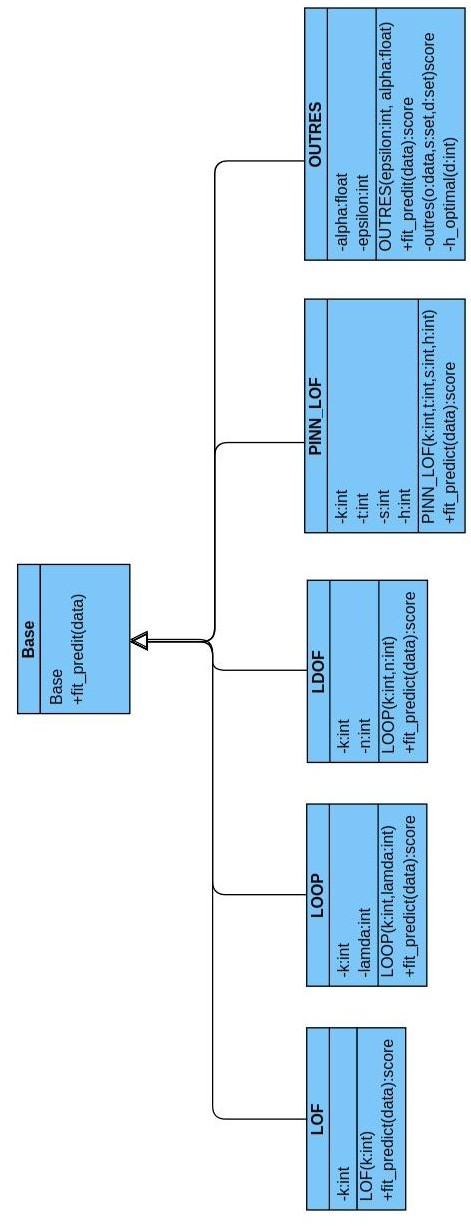
\includegraphics[width=\textwidth,height=\textheight]
    {imagenes/esquema.jpg}}
    \caption{\label{fig:esquema} Diagrama de clases}
\end{figure}

Como podemos ver todos nuestros algoritmos implementan la clase abstracta
\texttt{Base}. Por tanto, para poder utilizar cualquier algoritmo bastaría
con crear un objeto de la clase deseada y los parámetros elegidos. Después,
se usaría la función \texttt{fit predit(datos)} pasando como parámetro 
los datos a analizar.


%
\chapter{Implementación}
En este capítulo vamos a pasar a explicar con 
total detalle cada uno de los algoritmos implementados.
Explicaremos tanto sus fundamentos, como su motivación
y por último la implementación que se ha llevado a cabo.

\section{LOF}
Para el desarrollo y implementación de este algoritmos se 
ha utilizado como referencia tanto el libro \cite{aggarwalOutlierAnalysis2017}
como el artículo donde se presenta el algoritmo \cite{breunigLOFIdentifyingDensitybased2000}.


Local Outlier Factor (LOF), o en español factor de 
valor atípico local, es una cuantificación 
del valor atípico de un punto perteneciente al conjunto de datos.
Esta cuantificación es capaz de ajustar las variaciones
en las densidades locales. De modo que el objetivo será obtener 
una puntuación a través del análisis de densidad local a cada punto.
Para el cálculo de dicha puntuación vamos a desarrollar varias 
definiciones necesarias para comprender el desarrollo


En primer lugar, para un dado punto $\overline{X}$,
definimos $D^k(\overline{X})$ como la distancia del 
k-vecino más cercano de $\overline{X}$. Normalmente
el conjunto de puntos que se encuentran a una distancia
$D^k(\overline{X})$ de  $\overline{X}$ contiene k puntos.
Esto no es estrictamente necesario ya que podemos tener puntos
a la misma distancia exacta y por tanto tener más de k
puntos.


Ahora podemos definir la reachability distance o distancia de
alcance en español, del punto  $\overline{X}$ con respecto
del punto  $\overline{Y}$: 

\begin{center}
    $R_k(\overline{X},\overline{Y}) = max ( dist(\overline{X},\overline{Y}), D^k(\overline{X}) ) $
\end{center}

La distancia de alcance, como podemos imaginar no es simétrica
entre $\overline{X}$ y $\overline{Y}$ ya que el k-vecino más cercano
de  $\overline{Y}$ puede ser otro totalmente distinto al de 
$\overline{X}$. Cuando $\overline{Y}$ está en una región densa y la
distancia entre $\overline{X}$ y $\overline{Y}$ es amplia, la distancia
de alcance de $\overline{X}$ usará la distancia entre ambos puntos $dist(\overline{X},\overline{Y})$. 
Por otro lado, cuando la distancia entre ambos puntos sea pequeña, la distancia de
alcance se suaviza con la distancia al k-vecino más cercano. Cuanto mayor
sea el valor de k mayor será el suavizado aplicado.


El cálculo de esta distancia se hace visible en la siguiente figura 
del artículo  \cite{breunigLOFIdentifyingDensitybased2000}: 

\begin{figure}[h]
    \center{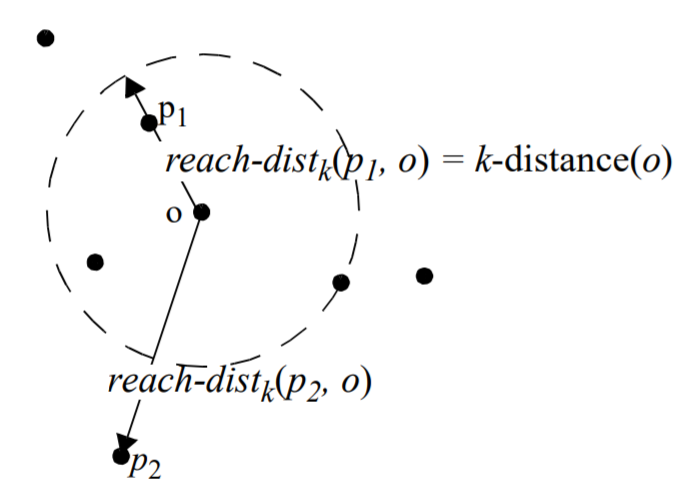
\includegraphics[width=\textwidth]
    {imagenes/distancia-alcance.png}}
    \caption{\label{fig:base-abstraccion} Abstracción de la clase general sklearn}
\end{figure}

Ahora podemos definir la media de la distancia de alcance $AR_k$, teniendo
en cuenta que el conjunto $L_k(\overline{X})$ es el conjunto de puntos a una
distancia menor que el k-vecino más cercano. 

\begin{center}
    $AR_k(\overline{X}) = MEDIA_{\overline{Y} \in L_k(\overline{X}) } R_k(\overline{X},\overline{Y})$
\end{center}

Aquí la media representa la media de valores de un conjunto de valores.
Con esta definición podemos definir el valor LOF


\begin{center}
    $LOF_k(\overline{X}) = AR_k(\overline{X}) \cdot MEDIA_{\overline{Y} \in L_k(\overline{X}) }       \frac{1}{AR_k(\overline{Y})} $
\end{center}

El uso de relaciones de distancia en la definición asegura que el
comportamiento de la distancia local se tenga en cuenta en esta definición.
Como resultado, los valores LOF para los objetos en un clúster
a menudo son cercanos a 1, cuando los puntos de datos en el clúster
se distribuyen de manera homogénea. Por ejemplo, en el caso de la 
figura \ref{fig:densidad}, los valores de LOF de los puntos de datos
en ambos grupos serán cercanos a 1, aunque las densidades de los dos 
grupos sean diferentes.

El cálculo de LOF puede ser visto como una normalización de la distancia
de alcance de un punto, donde el factor de normalización usado es la 
media armónica. Ambos casos son en principio válidos, aunque nosotros usaremos
la primera definición por simplicidad e interpretación.


Por otro lado, cabe mencionar que LOF también puede considerarse como
un algoritmo basado en distancias relativamente con suavizado. Se calculan
las distancias entre puntos para el cálculo de la distancia de alcance.
Como ya mencionábamos podemos dar ciertos enfoques ya que usan conceptos
de los tres tipos de algoritmos que comentábamos en el capitulo 
\ref{cap:Analisis}.

Aquí tenemos el pseudocódigo del algoritmo LOF. En nuestro caso implementado
en Python y haciendo el máximo uso posible de estructuras de datos eficientes,
para conseguir una implementación veloz y eficiente.

\begin{codigo}
    \begin{algorithmic}[1]
    \Function {LOF}{Matrix de datos D, k}
    \State \parbox[t]{305pt}{distancias = calcular matrix de distancias con k-nn}
    \ForEach{$x_i \in \mathcal D $}
    \State \parbox[t]{305pt}{ $AR_k(x_i) = MEDIA_{y \in L_k(x_i) } R_k(x_i,y)$}
    \State {$LOF_k(x_i) = AR_k(x_i) \cdot MEDIA_{y \in L_k(x_i) }       \frac{1}{AR_k(y)} $}
    \EndFor 
    \State \Return Puntuaciones: $LOF_k$
    \EndFunction 
    \end{algorithmic}
\end{codigo}


\section{LOOP}
Esta técnica combina varios conceptos. en primer lugar, la idea de localidad,
los algoritmos basados en densidad como LOF. Por otro lado, LOCI con conceptos
probabilísticos para modelar la puntuación de una anomalía. Un enfoque probabilístico 
significa ofrecer una tolerancia natural a los efectos de ruido en los datos. 
Los enfoques tradicionales como LOF y LOCI pueden incluso enfatizar tales efectos. 
Por ejemplo, LOF se basa en comparar las k distancias de los puntos, es decir, 
las distancias de los puntos a su k-vecino más cercano. Una elección inapropiada 
(localmente) de k puede causar resultados malos como ya comentamos anteriormente.

En esta técnica se propone una puntuación que incluye una normalización para 
convertir en independiente de la distribución de datos específica en un conjunto 
de datos dado, así como una motivación estadísticamente sólida para obtener valores 
en el rango de [0, 1], fácilmente interpretable como la probabilidad de un 
determinado punto en ser una anomalía.

Vamos a explicar detalladamente este nuevo enfoque el cual podemos encontrar con 
más detalle en el artículo de referencia \cite{kriegelLoOPLocalOutlier2009}. 
Seguiremos la misma notación del artículo para conseguir una comprensión 
más fácil.

Asumimos como $D$ el conjunto de datos con $n$ puntos o objetos y $d$ dimensiones.
Ahora definimos el concepto de distancia probabilística de un objeto $ o \in D$ 
en un contexto de $S \subseteq D$ y a la cual nos referimos como $pdist(o,S)$. 
Esta distancia se define como:

\[ 	\forall s \in S: P[d(o,s) \leq pdist(o,S)] \geq \varphi  \]

Intuitivamente, estamos cogiendo una esfera alrededor de $o$ con radio $pdist $
cubre cualquier elemento en el conjunto de contexto $S$ con una probabilidad de
$\varphi$. La distancia probabilística $pdist (o, S)$ de $o$ a $S$ se puede 
interpretar como la extensión estadística del conjunto de contexto S. La principal 
diferencia con la extensión (normal) de un conjunto de puntos es que la extensión 
estadística permite deliberadamente algún error. El recíproco de la distancia 
probabilística puede verse como una estimación de la densidad:

\[ 	pdens(S) = \frac{1}{pdist(o,S)} \]

Podemos simular la noción estadística clásica y sólida de valores atípicos
definidos como objetos que se desvían más de un $\lambda$ dado la desviación
estándar $\sigma$ de la media. Para ello usamos la siguiente difinición de $\lambda$

\[ 	 \lambda = \sqrt{2} \cdot erf^{-1}(\varphi) \]

Donde $erf$ representa la función de error Gaussiana. Esto nos permite determinar
nuestro error a través de los diferentes valores de $\lambda$.


Asumiendo que o se encuentra en el centro de $S$ podemos calcular la desviación 
estándar como:

\[ \sigma(o,S) = \sqrt{ \frac{\Sigma_{s \in S} d(o,s)^2 }{|S|} }    \]

Con estas consideraciones podemos redefinir la distancia probabilística con
la siguiente expresión:


\[ pdist(\lambda,o,S) := \lambda \cdot \sigma(o,S) \]

Intuitivamente, esta distancia de conjunto probabilístico estima la densidad 
alrededor de $o$ en función de $S$. El parámetro $\lambda$ da control sobre 
la aproximación de la densidad. Sin embargo, es solo un factor de normalización 
que solo afecta el contraste en las puntuaciones resultantes. La clasificación 
de los valores atípicos no se verá afectada por $\lambda$.

Para el correcto funcionamiento de esta técnica debemos realizar varias suposiciones.
La más importante es que estamos suponiendo que el conjunto $S$ esta centrado $o$.
Esta suposición no es fácil de conseguir ya que estamos conformando el conjunto $S$
como una distancia radio. Esto nos da ciertas ventajas y es que la técnica combina
la ventaja de dos mundos, los enfoques basados en densidad que no asumen 
ninguna distribución de datos específica y los conceptos matemáticos 
sólidos de los métodos estadísticos. Con estas razones y teniendo en cuenta que 
$E[  \; ]$ se refiere a la media definimos el factor local de anomalía o LOF probabilístico:

\[ PLOF_{\lambda,S}(o) := \frac{pdist(\lambda,o,S(o))}{E_{s \in S(o)} [pdist(\lambda,s,S(s))]} -1 \] 


El valor $PLOF$ de un objeto $o \in D$ calcula la relación de la 
estimación para la densidad alrededor de $o$ que se basa en $S(o)$ 
y el valor esperado de las estimaciones para las densidades alrededor 
de todos los objetos en el conjunto de contexto $S(o)$
Debemos de resaltar que a pesar de obtener valores parecidos a los de LOF,
estos no son aun probabilidades ni están normalizados.

Para lograr una normalización que haga que la escala de PLOF sea 
independiente de la distribución de datos en particular, el valor 
agregado nPLOF se obtiene con la siguiente expresión:

\[ nPLOF := \lambda \cdot \sqrt{E[PLOF^2]}\]

Este valor puede verse como un tipo de desviación estándar de
valores PLOF.

Ahora aplicamos la Función de Error Gaussiana (erf) para obtener 
un valor de probabilidad, el \textbf{Local Outlier Probability (LoOP)}

\[ LoOP(o) := max ( 0, erf( \frac{PLOF_{\lambda,S}(o)}{nPLOF \cdot \sqrt{2}})    )\]


El valor de LoOP estará cerca de 0 para puntos dentro de regiones densas 
y cerca de 1 para valores atípicos basados en densidad local.
En otras palabras, si bien una puntuación de valores atípicos de $x$ 
calculada por un enfoque local como LOF designará diferentes grados 
de valores atípicos para diferentes regiones del mismo conjunto de 
datos y no se puede comparar con una puntuación de $x$ en un conjunto 
de datos diferente, los valores de LoOP son consistentes sobre el
conjunto completo de datos y en múltiples conjuntos de datos. El resultado
es una probabilidad de ser anomalía en el intervalo [0-1], por lo que 
podemos comparar entre cualquier conjunto de datos.
Esto nos aporta una mejor interpretabilidad de los resultados frente a otros
métodos.

Vamos ahora a exponer el pseudocódigo de este algoritmo y el usado para su
implementación en nuestra biblioteca. En primer lugar, debemos comentar que
hemos usado el algoritmo k-nn como base para construir los conjuntos S,
asegurando de este modo que nuestro objeto o sea el centro del volumen.

\begin{codigo}
    \begin{algorithmic}[1]
    \Function {LOOP}{Matrix de datos D, k, $\lambda$ }
    \State \parbox[t]{305pt}{calcular matrix de distancias con k-nn y conjunto $S(o)$}
    \ForEach{$o \in \mathcal D $}
    \State \parbox[t]{305pt}{ $ \sigma(o,S) = \sqrt{ \frac{\Sigma_{s \in S} d(o,s)^2 }{|S|} } $}
    \State {$pdist(\lambda,o,S) := \lambda \cdot \sigma(o,S) $}
    \State {$PLOF_{\lambda,S}(o) := \frac{pdist(\lambda,o,S(o))}{E_{s \in S(o)} [pdist(\lambda,s,S(s))]} -1 $}
    \State {$nPLOF := \lambda \cdot \sqrt{E[PLOF^2]} $}
    \State {$LoOP(o) := max ( 0, erf( \frac{PLOF_{\lambda,S}(o)}{nPLOF \cdot \sqrt{2}})    ) $}
    \EndFor
    \State \Return Puntuaciones: $LOOP$
    \EndFunction 
    \end{algorithmic}
\end{codigo}

En nuestro caso al realizar una implementación en Python hemos usado la comprensión
de listas en lugar de un bucle for y de este modo conseguimos una mayor velocidad.
Con esto conseguimos que el algoritmo sea realmente útil reduciendo su tiempo
de computación.


\section{LDOF}
Esta técnica busca resolver el problema de la detección de anomalías cuando los 
datos que queremos analizar son dispersos. Muchas técnicas suponen que los datos
se agrupan en unos pocos grupos, pero en los datos reales existen multitud de conjuntos
de datos donde los puntos se presentan dispersos.


Local Distance-based Outlier Factor (LDOF) o Factor de Factor de valores atípicos 
basados en la distancia local en español, es sensible a los valores atípicos en 
conjuntos de datos dispersos. LDOF utiliza la distancia relativa de un 
objeto a sus vecinos para medir la cantidad de objetos que se desvían de 
su vecindario disperso. Cuanto más alto es el grado de violación que 
tiene un objeto, más probable es que el objeto sea un valor atípico. 
Para simplificar la configuración de parámetros en aplicaciones del mundo
real, la técnica top-n se emplea en este enfoque.

Como referencia para el desarrollo de este algoritmo 
se ha usado el artículo donde los autores los presentan \cite{zhangNewLocalDistancebased2009}

La motivación de este algoritmo nace de la ineficiencia de algoritmos como
k-nn o LOF en datos dispersos. Para ver este hecho vamos a mostrar un ejemplo
donde esto se hace visible. Usamos el ejemplo que plantean los autores:

\begin{figure}[h]
    \center{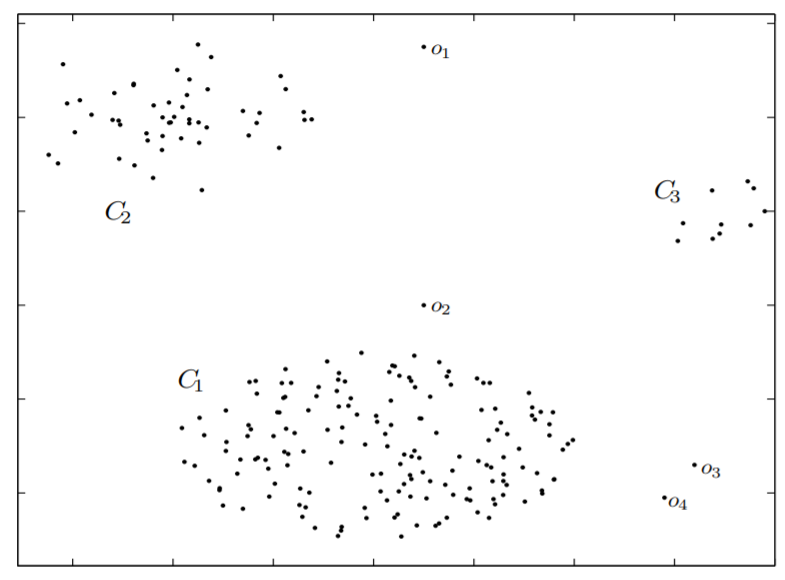
\includegraphics[width=\textwidth]
    {imagenes/datos-dispersos.png}}
    \caption{\label{fig:datos-dispersos} Ejemplo de datos dispersos}
\end{figure}

Analizamos el comportamiento de k-nn, cuando k es mayor 
que la cardinalidad de C3 (10 en este caso), algunos objetos en C1 se 
convierten en vecinos de los objetos en C3. Por lo tanto, la distancia 
del objeto puede ser mayor que los valores atípicos.
En el caso de LOF, ya que la densidad de C3 es más pequeña que la de C1,
la clasificación de o1, o2, o3 y o4$o_1, o_2, o_3, o_4$ 
como valores atípicos se complica y puede ser errónea.
Por tanto, en nuestro enfoque la idea principal será medir cómo 
un objeto se desvía de su sistema de vecindad como un factor de valor 
atípico.


Ahora vamos a explicar las definiciones y cálculos necesarios para la obtención
final de la puntuación. Para mantener la coherencia con el artículo de referencia
mantendremos la misma anotación. Definimos $N_p$ como el conjunto de los k-vecinos
más cercanos del punto $x_p$, excluyéndolo del propio conjunto. Definimos
la distancia de k-vecinos más cercanos como:


\[ \bar{d}_{x_p}  := \frac{1}{k} \sum_{x_i \in N_p} dist(x_i,X_p)\]

Ahora definimos la distancia interna de $x_p$ como la distancia promedio 
entre los objetos en $N_p$

\[     \bar{D}_{x_p}  := \frac{1}{k(k-1)}  \sum_{x_i,x_i'  \in  N_p i \neq i' }   \]


Finalmente se define el factor de valor atípico basado en la distancia local 
(LDOF)de $x_p$ como:
\[    LDOF_k(x_p) := \frac{\bar{d}_{x_p}}{\bar{D}_{x_p}}       \]

\begin{figure}[h]
    \center{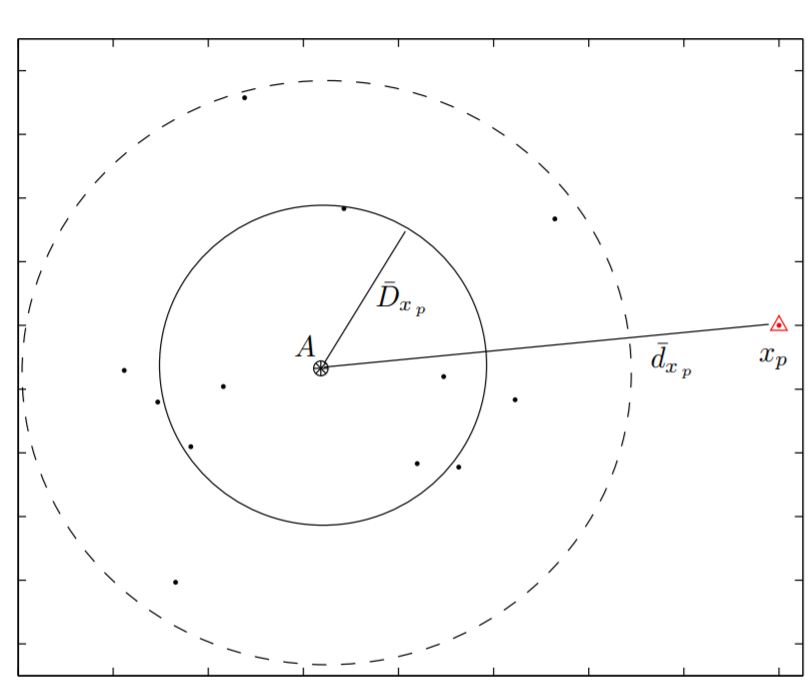
\includegraphics[width=\textwidth]
    {imagenes/LDOF.png}}
    \caption{\label{fig:LDOF} Ejemplo de funcionamiento de LDOF}
\end{figure}

La definición de LDOF, como se muestra en la Figura \ref{fig:LDOF}, 
claramente considera que $x_p$ está fuera de su región de vecindario. 
El valor LDOF de $x_p$ es obviamente mayor que 1, lo que indica que $x_p$
es un valor atípico. A través de este ejemplo, podemos ver que LDOF 
puede capturar efectivamente la condición de anomalía de un objeto 
entre un vecindario disperso. Además, a medida que k crece, LDOF 
toma más objetos en consideración y la vista de LDOF se vuelve cada 
vez más global. Si un objeto está lejos de su gran sistema de vecindad, llevado al 
extremo todo el conjunto de datos, es definitivamente un valor 
atípico. Por lo tanto, la precisión de detección del método podría ser
estable en un amplio rango de k.

\begin{codigo}
    \begin{algorithmic}[1]
    \Function {LDOF}{Matrix de datos D, k }
    \State \parbox[t]{305pt}{calcular matrix de distancias con k-nn}
    \ForEach{$X_p \in \mathcal D $}
    \State \parbox[t]{305pt}{ $ \bar{d}_{x_p}  := \frac{1}{k} \sum_{x_i \in N_p} dist(x_i,X_p) $}
    \State {$\bar{D}_{x_p}  := \frac{1}{k(k-1)}  \sum_{x_i,x_i'  \in  N_p i \neq i' }$}
    \State {$PLOF_{\lambda,S}(o) := \frac{pdist(\lambda,o,S(o))}{E_{s \in S(o)} [pdist(\lambda,s,S(s))]} -1 $}   
    \State {$ LDOF_k(x_p) := \frac{\bar{d}_{x_p}}{\bar{D}_{x_p}} $}
    \EndFor
    \State \Return Puntuaciones: $LDOF_k$
    \EndFunction 
    \end{algorithmic}
\end{codigo}

Este es el pseudocódigo usado para la implementación en nuestra biblioteca.
Al igual que pasaba con LDOF el bucle queda eliminado con el uso de la 
comprensión de listas de Python por motivos de eficiencia.


\section{PINN-LOF}
Esta técnica nace a partir de la idea de que existen áreas de 
aplicación en las que se encuentran con frecuencia problemas de 
rendimiento debido al gran tamaño de los conjuntos de datos y las 
dimensiones incluyen texto y datos médicos, para los cuales aún no 
se han investigado adecuadamente los beneficios potenciales del 
análisis de valores atípicos locales. En general, las dificultades 
de escalabilidad inherentes generalmente impiden el uso de técnicas 
de valores atípicos locales estándar para obtener resultados útiles 
en conjuntos de datos tan grandes y de gran dimensión. Esta técnica
se presenta en el siguiente artículo \cite{vriesFindingLocalAnomalies2010}

El mayor desafío es cómo lidiar con la 'maldición de la dimensión:
a medida que la dimensión de los datos crece, las medidas de 
distancia pierden su capacidad discriminativa, y las técnicas de 
indexación convencional ya no son efectivas para administrar la 
búsqueda de vecinos requerida por los métodos basados en distancias y 
densidad.


Existen varias técnicas para intentar mitigar estos problemas como el uso
de estrategias de sampling o métodos de indexación con poda. Aunque estas
quedan muy limitadas a casos específicos.

En este algoritmo se propone un método de detección de valores 
atípicos locales proyectivo basado en LOF, al que llamamos Vecino 
Más Cercano Indexado por Proyección, Más conocido por su nombre en
ingles Projection-Indexed Nearest-Neighbour (PINN).

PINN va más allá de la estrategia simple de 'proyectar y computar',
calcula las distancias requeridas por LOF al calcularlas dentro de 
un espacio de proyección de dimensiones reducidas, donde se puede 
esperar que los costos computacionales asociados con la búsqueda 
del vecino más cercano sean significativamente más pequeños que en 
el espacio original. También se plantea que cuando la matriz de 
proyección se determina aleatoriamente, el error de estimación de 
LOF puede limitarse con una probabilidad muy alta.

El primer problema a resolver que surge es que cuando realizamos una
proyección aleatoria no podemos garantizar que los valores que íbamos
a obtener para un punto $p$ con $LOF(p)$ se mantengan al calcular
$LOF(p')$. Veamos cómo podría afectarnos el realizar una proyección
aleatoria en la siguiente figura:


\begin{figure}[h]
    \center{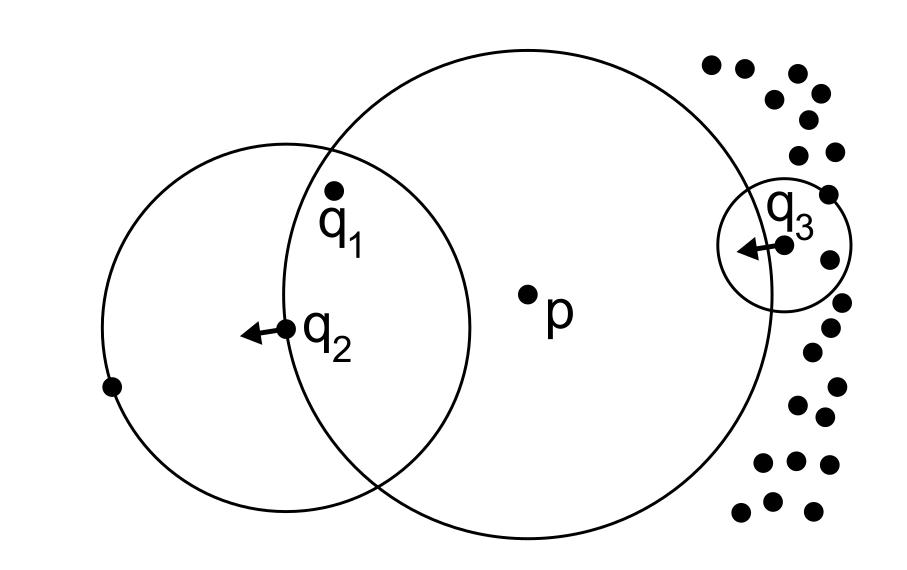
\includegraphics[width=\textwidth]
    {imagenes/aleatoria.jpeg}}
    \caption{\label{fig:aleatoria} Ejemplo de situación para proyección aleatoria}
\end{figure}

Después de la proyección, $p$ tendría $q_3$ como vecino en lugar de $q_2$, 
lo que resultaría en un aumento sustancial en la densidad relativa 
asociada con ese vecino. Si muchos vecinos son reemplazados de esta 
manera tendríamos un cambio considerable en los resultados finales.

Como alternativa a la estimación de $LOF(p)$ por $LOF(p')$, en su
lugar se propone que el cálculo de $LOF(p)$ se calcule en él, 
espacio original, pero se calcule utilizando el vecindario 
y distancias de vecindario según lo determinado después de la 
proyección.


La idea por tanto será, en lugar de pagar el alto costo del cálculo 
del k-vecino más cercano en el espacio original, podemos determinar 
un vecindario más grande dentro del espacio de proyección e 
invertir el mapeo para obtener estimaciones de los vecinos en el 
espacio original. Si se considera un número suficiente de vecinos 
en el espacio de proyección (donde el número depende de la dimensión 
intrínseca de $D'$), el verdadero conjunto original de k-vecinos se 
puede recuperar con muy alta probabilidad. Esto nos supondría una 
alta reducción de coste computacional. Veamos las etapas en la siguiente
figura que nos proporciona el artículo de referencia \cite{vriesFindingLocalAnomalies2010}


\begin{figure}[H]
    \center{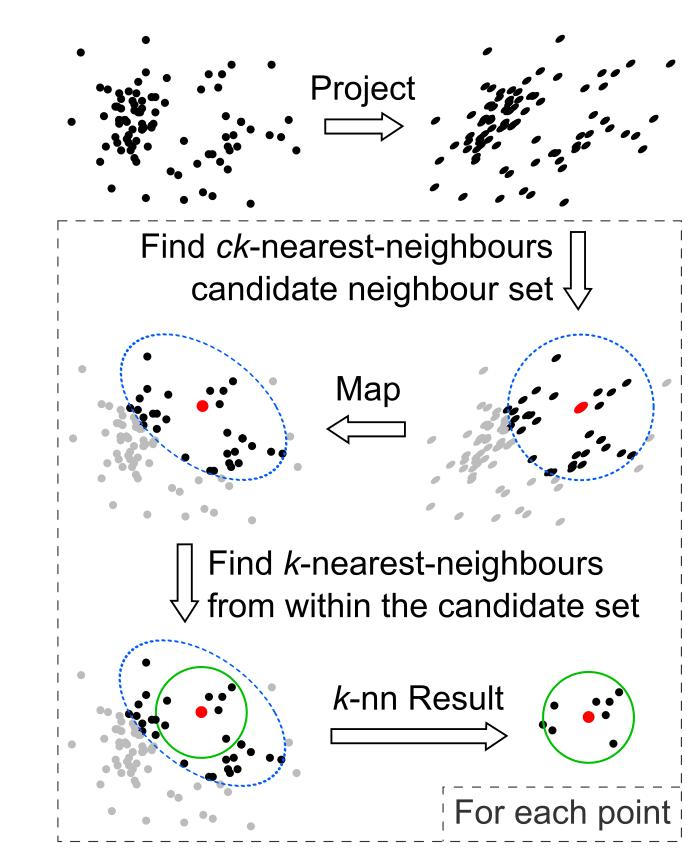
\includegraphics[width=\textwidth]
    {imagenes/etapas-pinn.jpeg}}
    \caption{\label{fig:pinn} Etapas del algoritmo PINN}
\end{figure}

Con estos resultados y teniendo calculado el conjunto de los k-vecinos
más cercanos, en nuestro caso usaremos $LOF$ para el cálculo final de
las puntuaciones.

Vamos a exponer el pseudocódigo del algoritmo para entender mejor su funcionamiento:

\begin{codigo}
    \begin{algorithmic}[1]
    \Function {RP+PINN+LOF}{Matrix de datos D,k,t,s,h }
    \State \parbox[t]{305pt}{\textbf{RP:} Realizamos una projección aleatoria $D \rightarrow Y$}
    \State \textbf{PINN}: h define el tamaño del set de candidatos.
    
    \ForEach{$p \in \mathcal D $}
    \State \parbox[t]{305pt}{ 1) encontrar los h-vecinos más cercanos en el espacio $y$}
    \State {2) Mapeamos el vecindario calculado con los puntos en el espacio original $D$}
    \State {3) Calculamos los k-nn vecinos más cercanos para $p$ dentro del vecindario}   
    \EndFor
    \State \textbf{LOF}: Aplicamos $LOF$.
    \State \Return Puntuaciones: $LOF$
    \EndFunction 
    \end{algorithmic}
\end{codigo}


Como podemos ver, a pesar de que intrínsecamente estamos usando $LOF$ como
sistema de puntuación de anomalías, la idea es crear un proceso para permitir
su aplicación en dimensiones superiores sin caer en la maldición de la
dimensionalidad. De este modo tenemos un proceso efectivo y rápido. En 
nuestro caso al realizar una implementación en Python hemos aprovechado 
al máximo las herramientas de este lenguaje para buscar la máxima eficiencia.

\section{OUTRES}
Para el desarrollo de este algoritmo hemos usado como referencia el
artículo donde se desarrolla con máximo detalle \cite{mullerAdaptiveOutliernessSubspace2010}

Esta técnica nace a partir de una idea clara, en las técnicas tradicionales
se establecen las anomalías a través del uso de todo el espacio. Pero de ese
modo nos estamos perdiendo lo que hay escondido en las proyecciones de subespacios.
Por tanto, la propuesta es desarrollar una puntuación de anomalías basada 
en la desviación de objetos en las proyecciones subespaciales. Principalmente
se centra en obtener la puntuación midiendo su grado de desviación local.
Además, solo se hará uso de un subconjunto de atributos y no del espacio
completo, y es que un objeto puede mostrar una alta desviación en 
comparación con su vecindario en un subespacio. Además, el mismo 
objeto puede agruparse con otros objetos en un segundo subespacio y 
puede no aparecer como un valor atípico. O por otro lado aparecer en 
un tercer subespacio disperso donde todos los objetos parecen ser 
valores atípicos. Veamos un ejemplo de esto en la siguiente figura:


\begin{figure}[h]
    \center{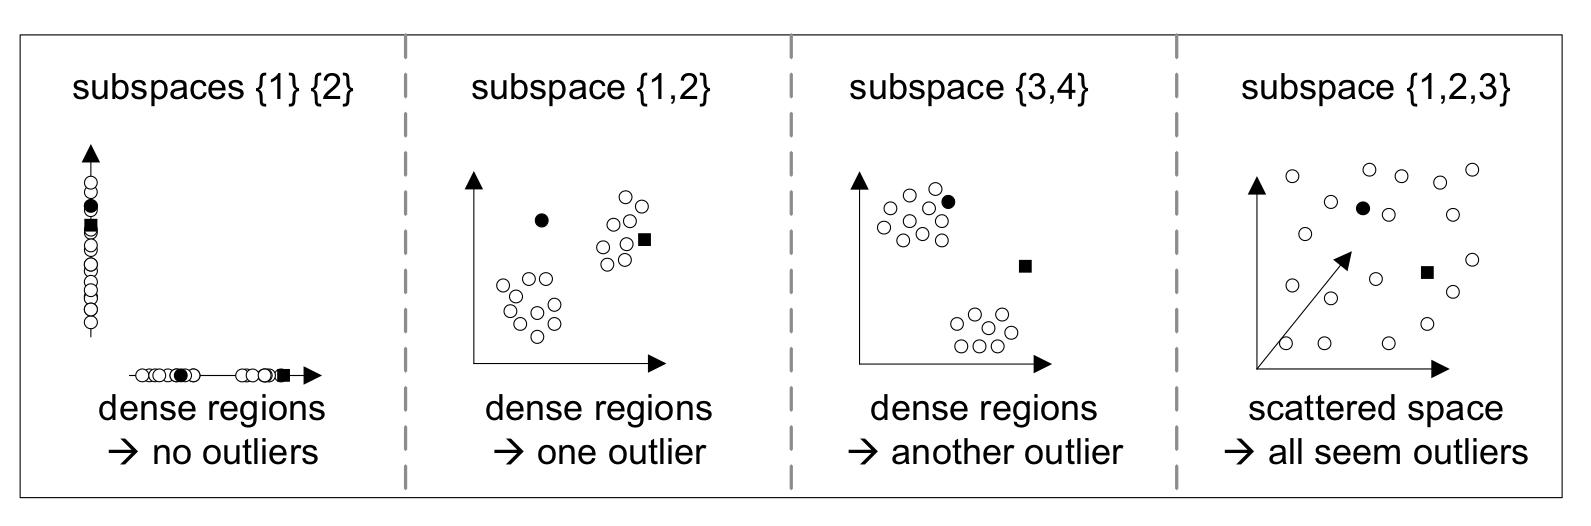
\includegraphics[width=\textwidth]
    {imagenes/subespacios.jpeg}}
    \caption{\label{fig:subespacios} Anomalías en diferentes subespacios}
\end{figure}

Como podemos ver es posible que cada anomalía necesite una proyección para
poder detectarla de forma clara. Las técnicas de reducción de dimensionalidad 
global, como el análisis de componentes principales PCA, proporcionan 
una única proyección para todos los objetos. En contraste, nuestro objetivo es 
detectar múltiples subespacios relevantes por objeto. La agrupación en subespacio 
detecta múltiples proyecciones, sin embargo, se centra en subespacios para grupos 
de objetos agrupados. Para la clasificación de valores atípicos, el enfoque está 
en los objetos y subespacios individuales en los que un valor atípico se desvía 
mucho de su vecindario local. Un enfoque muy novedoso.


El método se basa en dos pilares principalmente. Primero, para cada objeto, 
seleccionamos estadísticamente un conjunto de proyecciones para la puntuación 
de valores atípicos. En estas proyecciones interesantes, existe la posibilidad
de encontrar valores atípicos o aumentar su puntuación. Por otro lado, los subespacios
se distribuyen de forma uniforme por lo que no aportan información y pueden ser
ignorados. En segundo lugar, la desviación del objeto aumenta con el número de
atributos en un subespacio relevante. Las distancias entre objetos crecen cada vez
más con la maldición de la dimensionalidad. Por tanto, cuando crece la dimensionalidad
los puntos suelen a estar más dispersos.


El algoritmo que se propone basado en todos estos conceptos es OUTRES donde solo se
usaran una selección de proyecciones no distribuidas uniformemente. Además, ya que el
calculo de desviación se realiza en varios subespacios con diferente dimensión, se propone
un método adaptativo con el número de atributos para el cálculo del score en cada subespacio.

Para describir el procedimiento del algoritmo seguiremos la notación de \cite{mullerAdaptiveOutliernessSubspace2010}
para facilitar su complementación con el artículo. La primera idea que debemos de desarrollar es
la de cómo combinar los resultados de diferentes subespacios para un mismo punto.
Para ello se usa la expresión
\[ r(o) = \prod_{S \in RS(o)} score(o,S)  \]

Donde el conjunto $Rs(o)$ representa el conjunto de subespacios relevantes para el objeto
$O$. Como podemos ver se calcula una agregación de los resultados de cada subespacio.

A continuación, debemos de resolver la incógnita de como seleccionar los subespacios
relevantes para cada objeto $o$. En primer lugar, para determinar si es interesante se
realizara un test estadístico para comprobar si esta uniformemente distribuido. Si 
solo aplicamos esto, deberíamos de realizar dicho test a todos los subespacios posibles.
Pero para evitar esto definimos un subespacio como uniformemente distribuido si todos sus
componentes también son uniformemente distribuidos. Así descartamos un subespacio
tan pronto como al menos un atributo este uniformemente distribuido. Con esta técnica
podemos realizar una alta poda en el momento en el que detectamos un atributo uniforme.
Veamos cómo funciona en la siguiente figura: 

\begin{figure}[h]
    \center{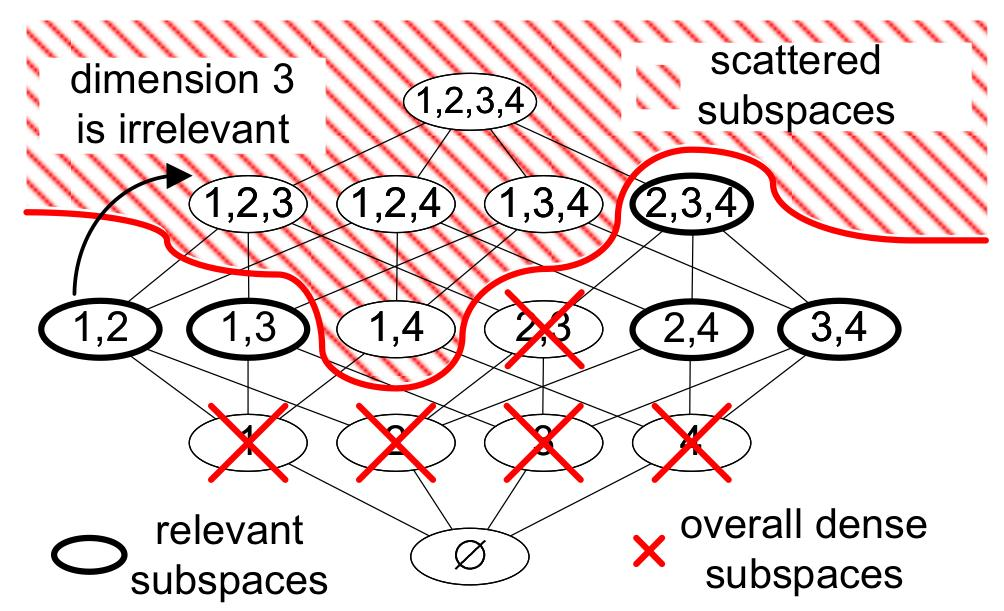
\includegraphics[width=\textwidth]
    {imagenes/seleccion-subespacios.jpeg}}
    \caption{\label{fig:select-subespacios} Selección de subespacios}
\end{figure}

En este caso conseguiríamos un gran coste computacional y no tendríamos que realizar los
test estadísticos ni ningún calculo más para aquellos subespacios que no aportan información.

Ahora vamos a explicar cómo se implementa el cálculo adaptativo de score para cada subespacio.
La idea es poder realizar un cálculo que permita su agregación independientemente de la 
dimensión del subespacio donde se está calculando.

Lo primero es plantear un vecindario adaptativo:

\[ AN(o,S) = \lbrack p | dist_S(o,p)= <= \epsilon(|S|) \rbrack  \]

La idea general es derivar el rango variable de una observación común en 
las proyecciones del subespacio. Mientras aumenta el número de atributos 
en una proyección subespacial, el volumen de un vecindario fijo disminuye 
significativamente en comparación con el volumen general del subespacio.

Ahora necesitamos una técnica para calcular la densidad en el vecindario,
que definimos como 

\[ den(o,S) = \frac{1}{|DB|} \sum_{p \in DB} K_e ( \frac{dist_S(o,p)}{h} ) \]

Donde $k_e$ es una función kernel en nuestro caso el kernel de Epanechnikov
que se define como

\[ K_e(x) = (1-X^2), x < 1\]

y definimos h como el parámetro de ancho de banda que se usa para escalar 
la influencia de cada objeto a una distancia máxima de h. Existe una expresión
para calcular el h optimo la cual se ha implementado y tiene en cuenta el volumen
de la dimensión como comentábamos antes que era importante.

Con esta h optima ya que se tiene en cuenta el volumen del subespacio como comentábamos
en la definición del vecindario adaptativo, podemos usarlo para el cálculo del tamaño
de dicho vecindario:


\[ \epsilon(|S|) = \epsilon \cdot \frac{h_{optimal}(|S|)}{h{optimal}(2)} \]


Por lo tanto, simplemente escalamos el ancho de banda inicial dado del espacio 2d 
al espacio de datos completo y utilizamos estos valores para la estimación de 
densidad. Ahora solo necesitamos calcular la desviación de la densidad.

\[dev(o,S) = \frac{\mu - den(o,S)}{2 \cdot \sigma} \]

Donde $\mu$ representa la media de la densidad y $\sigma$ la desviación estándar.

A pesar de que exista desviación solo la usaremos como score si dicha desviación es
significativa. De modo que ya tenemos todas las herramientas para definir nuestra función
de puntuación como:

\[ score(o,S) = \left\{ \begin{array}{lcc}
    \frac{den(o,S)}{dev(o,S)} si  dev(o,s) >=1 \\
    \\ 0 
    \end{array}
\right.\]

Como podemos ver es un proceso complejo el de selección de subespacios y análisis de 
cada subespacio. Como veíamos que los subespacios se componían de forma combinatoria,
una buena forma para implementar este algoritmo será con un enfoque recursivo. Aquí podemos
ver una descripción de OUTRES:



\begin{codigo}
    \begin{algorithmic}[1]
    \Function {OUTRES}{o,S }    
    \ForEach{$i \in \mathcal D \setminus S $}
    \State \parbox[t]{305pt}{$ S' = S \cup \lbrace i \rbrace $}
    
    \If{$S'$ es relevante( realizar test estadistico)}
    \State $den(o,S') = \frac{1}{|DB|} \sum_{p \in DB} K_e ( \frac{dist_{S'}(o,p)}{h}$
    \State $dev(o,S') = \frac{\mu - den(o,S')}{2 \cdot \sigma}$
    \If{$dev(o,S') >= 1$ alta desviación}
    \State $r(o) = r(o) \cdot \frac{den(o,S)}{dev(o,S)} $  agregar score
    \EndIf
    \State \textbf{OUTRES}(o,S')
    \EndIf  
    \EndFor
    \EndFunction 
    \end{algorithmic}
\end{codigo}

Este algoritmo como podemos ver en planteamiento es muy interesante ya que usa la 
recursividad de llamadas para conseguir la combinatoria entre subespacios de forma
fácil. El problema que 
plantea es su complejidad que es de $O(2^n \cdot n^2)$ debido a la combinatoria entre
todos los posibles subespacios. Como sabemos este es el peor de los casos y si se consigue
que haya poda, la eficiencia será mucho mejor. Veremos en la práctica más adelante como
afronta esta complejidad dicho algoritmo.


\section{ODIN}
Se ha desarrollado el algoritmo ODIN, el cual se presenta en \cite{hautamakiOutlierDetectionUsing2004}. 
\textbf{Outlier Detection using Indegree Number (ODIN)} es un algoritmo que hace uso 
del grafico de los k-vecinos más cercanos. Por tanto, el objetivo será desarrollar un 
algoritmo que a partir del algoritmo de k-vecinos más cercano se realice una mejora que 
nos ofrezca un mejor desempeño.

Se propone un algoritmo para calcular las anomalías, como idea base partimos del  
grafo de k-vecinos más cercanos. En este grafo cada nodo es un vector de datos o  
un ejemplo de datos. Los bordes de conexión entre dos vértices $v_i$ y $v_j$ se produce 
si $v_j$ esta entre los k-vecinos más cercanos de $v_i$. Este razonamiento se aplica a todos 
los vértices y obtenemos el grafo knn. Con dicha definición el grafo es dirigido ya que 
podemos tener conexiones en un sentido, pero no en el contrario. Pensemos en el ejemplo de una 
anomalía y un punto en una región densa. Podemos tener conexión de la anomalía al punto pero  
muy probablemente no tengamos la conexión reciproca. Además, el grafo tendrá pesos para 
cada conexión, determinando la distancia entre los diferentes puntos. Como tenemos en cuenta 
los k-vecinos más cercanos sabemos a priori que cada vértice tendrá k conexiones. Para la construcción 
de este grafo será necesario el cálculo de todas las distancias entre puntos y por tanto, 
una complejidad de $O(n^2)$.

En nuestro caso, \textbf{ODIN} hace uso del concepto de k-vecinos más cercanos mutuos (MkNN).
Para ello se define que dos vértices serán vecinos mutuos si en el grafo knn existen  
las conexiones entre $v_i$ y $v_j$, y reciproca $v_j$ y $v_i$. Deben existir ambas para que 
exista conexión. De modo que este grafo es no dirigido y podemos seguir teniendo pesos con la 
distancia entre ambos vectores.

Con el uso del grafo de k-vecinos más cercanos mutuos tenemos una definición muy intuitiva de que
es una anomalía. Para explicar el razonamiento y ver un ejemplo más claro, podemos usar
un ejemplo ya visto con anterioridad.


\begin{figure}[h]
    \center{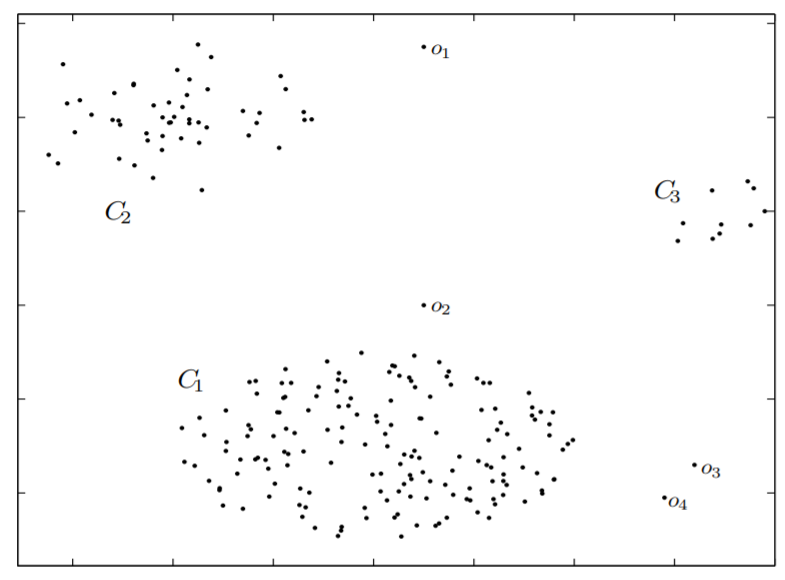
\includegraphics[width=\textwidth]
    {imagenes/datos-dispersos.png}}
    \caption{\label{fig:explica-knn} Ejemplo de anomalías}
\end{figure}


En este caso como podemos ver al generar los vecinos mutuos $O_1$ se quedaría sin vecinos 
ya que el resto de puntos de $C_2$ no lo considerarían como vecino mutuo. Por tanto, ya tenemos 
una definición intuitiva de outlier. Por un lado, los vértices con conexiones formarán 
clústeres mientras que los vértices sin conexiones serán las anomalías. 

En este ejemplo también podemos ver el problema que plantea esta definición. Pensemos en el  
punto $O_2$, es decir, un punto más cercano al clúster pero que es una anomalía. 
Puede entrar lo posibilidad de que algunos puntos del borde del clúster consideren al  
punto $O_2$ como un vecino mutuo y de este modo ya podría ser clasificado como un punto 
normal. Es necesario introducir cierta flexibilidad. Para ello en lugar de usar si tiene o no  
conexiones se usa el grado del vértice y se compara con un parámetro de entrada $T$ que funciona 
de umbral y podemos ajustar para ser más o menos restrictivos.

Ya tenemos los conceptos y la idea que sigue el algoritmo para detectar anomalías.
Vamos a plantear el procedimiento:


\begin{codigo}
    \begin{algorithmic}[1]
    \Function {ODIN}{S,k,T }  
    \State Calcular el grafo Mknn de S  
    \For{$i =1$ to $|S| $}
    \If{Grado de $v_i \leq T$ }
    \State \parbox[t]{305pt}{Marcar $v_i$ como anomalía}
    \EndIf  
    \EndFor
    \EndFunction 
    \end{algorithmic}
\end{codigo}


Como podemos ver el procedimiento es simple, primero calculamos el grafo
de vecinos mutuos y después con el grado de cada vértice determinamos si es
una anomalía si supera o no el umbral establecido por parámetro. 

  
Como podemos ver en este caso no realizamos el cálculo de ningún score si no que
se calcula una etiqueta binaria $0-1$ si es anomalía o no. Este tipo de resultado
ya lo explicamos anteriormente y aunque podríamos generar un score usando como
puntuación el grado de cada punto. En este caso hemos considerado interesante,
para ampliar la variedad de nuestra biblioteca, mantener la salida de etiqueta
binaria. De modo que mantenemos el enfoque de los autores.

  
Por otro lado, debemos mencionar que el parámetro $T$ puede plantear dificultades
para ajustarlo ya que realmente debemos de encontrar el umbral correcto y
será determinante para los resultados.


\section{MeanDIST y KDIST}
Vamos a tratar estos dos algoritmos en la misma sección ya que ambos se basan en
los mismos conceptos y se diferencian en el cálculo final. Los dos algoritmos parten 
de la idea expuesta en \cite{ramaswamyEfficientAlgorithmsMining2000} que se plasma 
en el algoritmo \textbf{RSS}.

Los conceptos que se plantean en \textbf{RSS} son muy básicos y fácil de comprender.
El algoritmo lo que hace es calcular los k-vecinos más cercanos y considerar anomalías
los $n$ puntos con las distancias a su k-vecino más grande. La idea es ordenar los puntos
por su distancia mayor en su vecindario y aquellos con distancias más grandes son aquellos
que no están en un clúster y, por tanto, anomalías. Como podemos ver el razonamiento es
fácil de comprender, pero presenta multitud de inconvenientes. En primer lugar, la definición
de anomalía puede no ser suficiente en multitud de casos, pero el principal problema 
es estimar $n$. Estamos suponiendo que a priori conocemos el número exacto de anomalías
que debemos detectar en los datos. Esto en la práctica no tiene funcionalidad.

A partir de esta idea y como mejora a los problemas que plantea, nacen los dos algoritmos
que analizamos en esta sección. En primer lugar el algoritmo \textbf{MeanDIST} usa
la media de las distancias en su vecindario para ordenar a los vértices. \textbf{KDIST} 
usará el máximo de las distancias a sus k-vecinos más cercanos. Hasta este punto no  
tenemos una mejora clara, pero la clave y la mejora reside en introducir un umbral como 
hacíamos en \textbf{ODIN} que sea más flexible y que además en este caso se calcule  
de forma inteligente.

Cuando analizamos la lista ordenada de distancias de menor a mayor, podemos comprobar
si la diferencia entre las distancias adyacentes es mayor que un determinado umbral $T$.
Para definir este umbral o punto de corte T usamos la siguiente ecuación

\[ T = max(L_i - L_{i-1}) * t \]

donde $L_i$ puede ser o la distancia calculada con \textbf{KDIST} o \textbf{MeanDIST}
del elemento i-ésimo. por otro lado $t$ será un valor entre $[0-1]$ que el usuario define 
por parámetro.

Para entender el cálculo del umbral veamos la siguiente figura que nos muestra la diferencia
entre los vectores ordenados.


\begin{figure}[h]
    \center{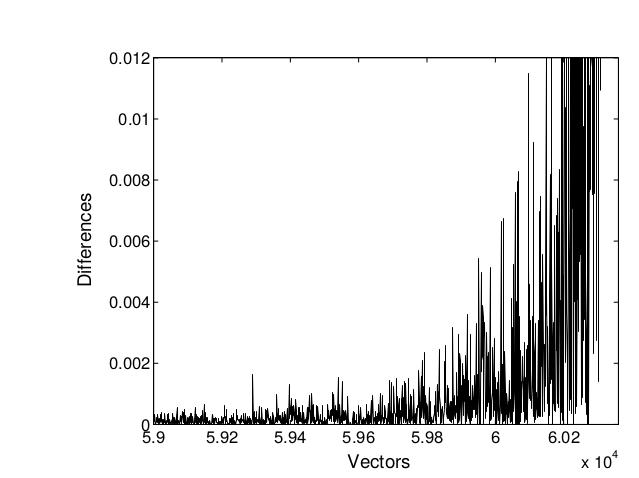
\includegraphics[width=\textwidth]
    {imagenes/salto-diferencia.jpeg}}
    \caption{\label{fig:explica-salto} Diferencia entre vectores ordenados por distancia}
\end{figure}


Como podemos ver existe un punto donde se produce un salto en la diferencia entre los vectores
ordenados. Aquí reside la definición de anomalía de estos dos algoritmos ya que podemos entender
que cuando se produce dicho salto estamos hablando de anomalías, vectores que se encuentran
muy distanciados del resto de datos. 

De modo que en el cálculo de este umbral estamos calculando en primer lugar la diferencia
más pronunciada que se produce en nuestros datos. Después establecer la amplitud de este
umbral y la permisión que admitimos con el parámetro $t$ definido por el usuario. 

Por tanto, con el cálculo del punto de corte entre los datos 
normales y las anomalías. Con estos conceptos definimos los algoritmos de la siguiente forma

\begin{codigo}
    \begin{algorithmic}[1]
    \Function {MeanDIST y KDIST}{S,k,t }  
    \State Calcular T
    \State Calcular el grafo knn de S
    \State L = vector ordenado ascendentemente
    \State Encontrar el i mas pequeño para el cual $ l_i - L_{i-1}  \geq T$
    \State Marcar como anomalia $L_i , ... , L_{|S|}$ 
    \EndFunction 
    \end{algorithmic}
\end{codigo}

La complejidad del algoritmo está marcada por el cálculo del grafo knn que conlleva
el cálculo de todas las distancias, es decir $O(n^2)$.
%
\chapter{Análisis experimental}
En este capítulo vamos a presentar las diferentes pruebas y la experimentación
realizada con los algoritmos implementados

\section{Pruebas de comportamiento}
En primer lugar, vamos a comentar las pruebas realizadas a cada algoritmo
para confirmar su correcto funcionamiento y para observar con más claridad
su comportamiento. Para ello todos los algoritmos han sido probados con un
conjunto de datos sintéticos. Este conjunto de datos se ha generado haciendo
uso del generador de numpy de números aleatorios. Para generar un conjunto
de datos con anomalías hemos usado una distribución estándar y hemos generado 
100 puntos de dimensión 2. Este conjunto de puntos se distribuye uniformemente
en la distribución seleccionada. Para generar anomalías vamos a generar 20
puntos que rompan con esta distribución. Para ello estos 20 puntos de dimensión
2 los generamos con una distribución uniforme. De este modo aseguramos que los 
los 20 puntos tienen una distribución diferente y podremos usarlos con anomalías.

Para ver el comportamiento de cada algoritmo vamos a mostrar los datos y 
alrededor de cada punto mostraremos un radio en función del score asignado a
cada punto. Para tener una medida más exacta y numérica de la efectividad del
algoritmo vamos a usar las curvas \textbf{ROC} y la métrica \textbf{AUC}.
Las curvas \textbf{ROC} enfrentan en una grafica la tasa de verdaderos
positicos $TPR$ con tra la tasa de falsos positivos $FPR$ donde ambos se definen como:

\[ TPR = \frac{VP}{VP + FN}\]

\[FPR = \frac{FP}{FP +VN}\]

La métrica \textbf{AUC} se cálcula como el área bajo la curva \textbf{ROC}. Proporciona 
una medición agregada del rendimiento en todos los umbrales de clasificación 
posibles. Una forma de interpretar el \textbf{AUC} es como la probabilidad de 
que el modelo clasifique un ejemplo positivo aleatorio más alto que un ejemplo 
negativo aleatorio.
Con esta métrica tenemos una medida muy eficiente del desempeño de nuestro
sistema ya que se tendrán en cuenta tanto los errores negativos como positivos.

También mencionar que se trata de un problema de clasificación desbalanceado por lo que
queremos poner el foco en la detección de las instancias anomalas sin aumentar la tasa
de falsos positivos.

En las siguientes figuras mostramos en primer lugar el desempeño observando el
radios. Para ver con más claridad los puntos que eran anomalías originalmente, 
estos están representados con un color diferente. Veamos el comportamiento de
los algoritmos implementados.




\begin{figure}[H]
    \begin{tabular}{cc}
      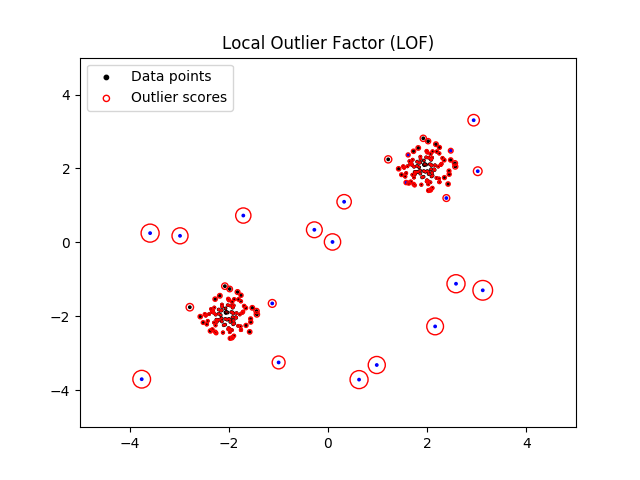
\includegraphics[width=65mm,height=40mm]{imagenes/lof-sintetico.png} &   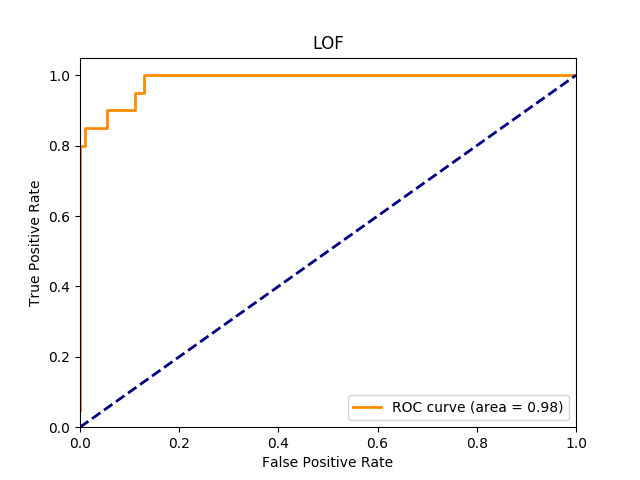
\includegraphics[width=65mm,height=40mm]{imagenes/lof-sintetic-roc.png} \\
    Score & Curca ROC para datos sinteticos \\[6pt]
    \multicolumn{2}{c}{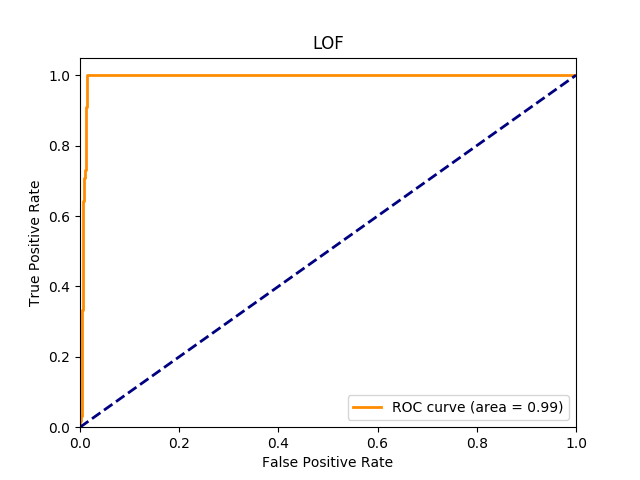
\includegraphics[width=65mm,height=39mm]{imagenes/lof-test.png} }\\
    \multicolumn{2}{c}{Curva ROC para datos reales}
    \end{tabular}
    \caption{\label{fig:loftest} LOF test}
\end{figure}

\begin{figure}[H]
    \begin{tabular}{cc}
      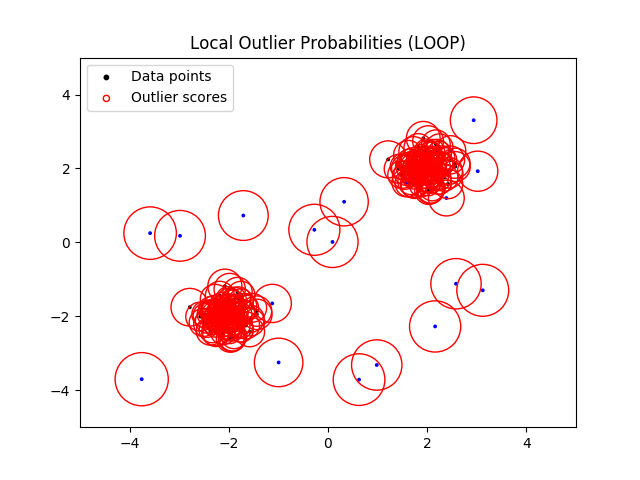
\includegraphics[width=65mm,height=40mm]{imagenes/loop-sintetico.png} &   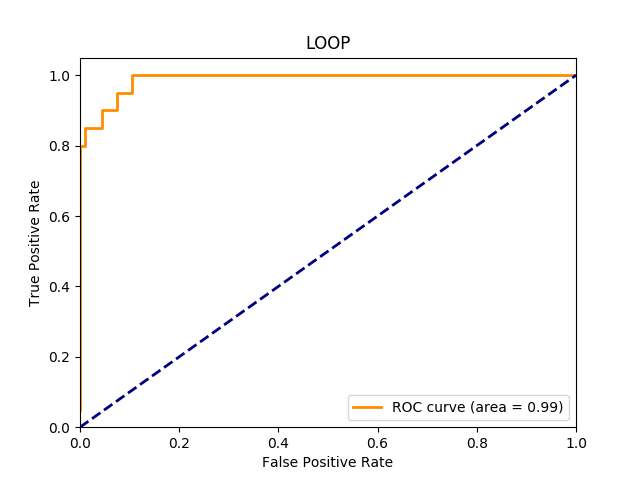
\includegraphics[width=65mm,height=40mm]{imagenes/loop-sintetic-roc.png} \\
    Score & Curca ROC para datos sinteticos \\[6pt]
    \multicolumn{2}{c}{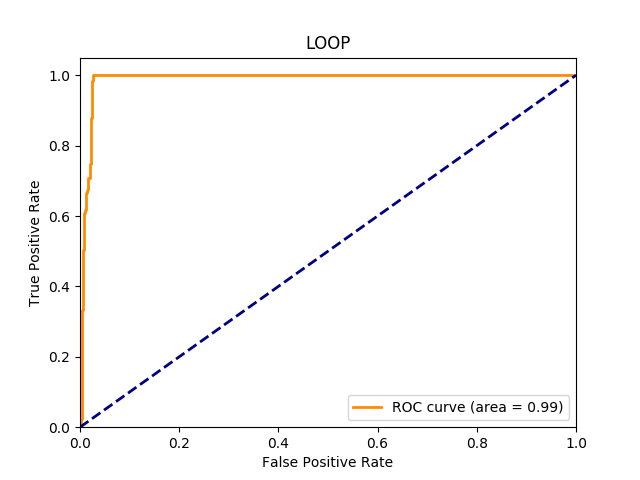
\includegraphics[width=65mm,height=39mm]{imagenes/loop-test.png} }\\
    \multicolumn{2}{c}{Curva ROC para datos reales}
    \end{tabular}
    \caption{\label{fig:looptest} LOOP test}
\end{figure}

\begin{figure}[H]
    \begin{tabular}{cc}
      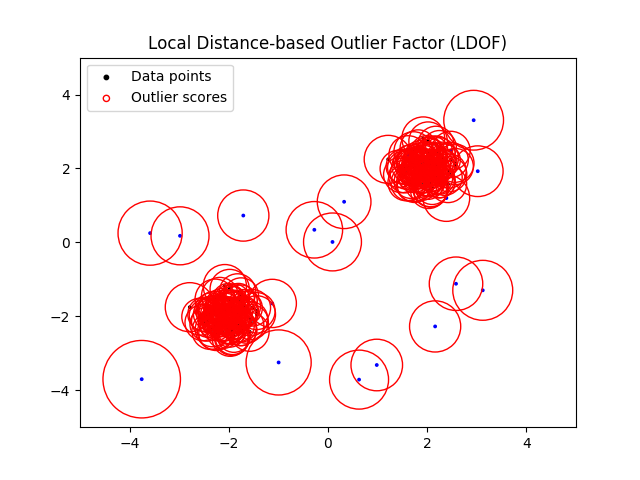
\includegraphics[width=65mm,height=40mm]{imagenes/ldof-sintetico.png} &   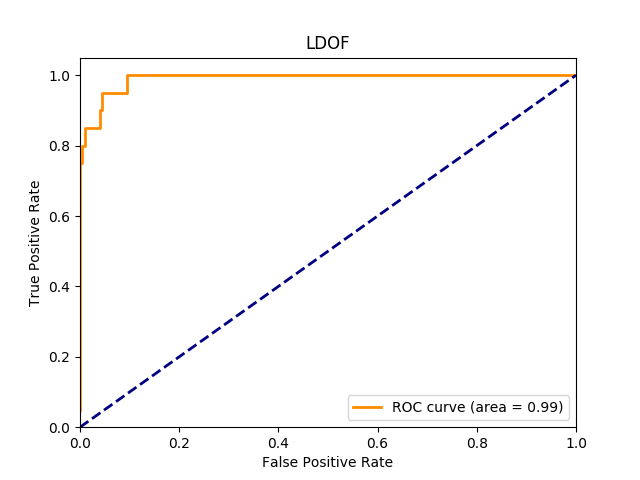
\includegraphics[width=65mm,height=40mm]{imagenes/ldof-sintetic-roc.png} \\
    Score & Curca ROC para datos sinteticos \\[6pt]
    \multicolumn{2}{c}{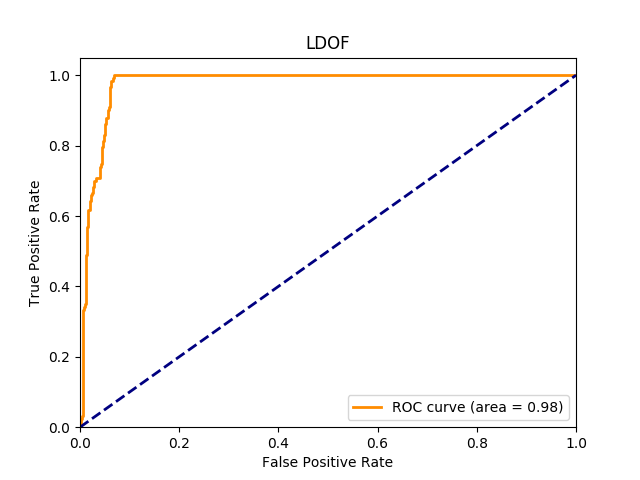
\includegraphics[width=65mm,height=39mm]{imagenes/ldof-test.png} }\\
    \multicolumn{2}{c}{Curva ROC para datos reales}
    \end{tabular}
    \caption{\label{fig:ldoftest} LDOF test}
\end{figure}

\begin{figure}[H]
    \begin{tabular}{cc}
      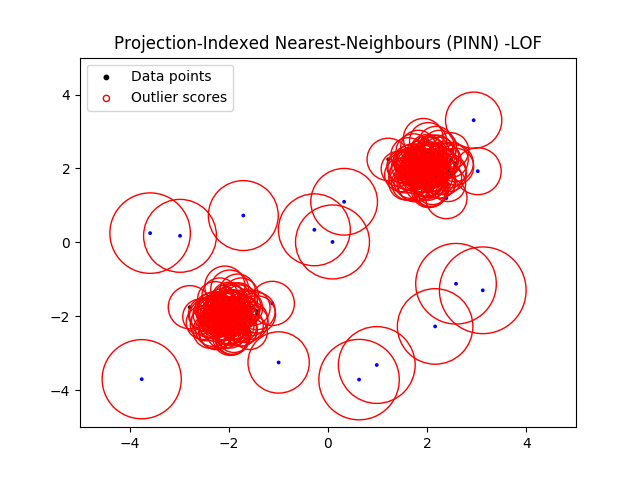
\includegraphics[width=65mm,height=40mm]{imagenes/pinn-lof-sintetico.png} &   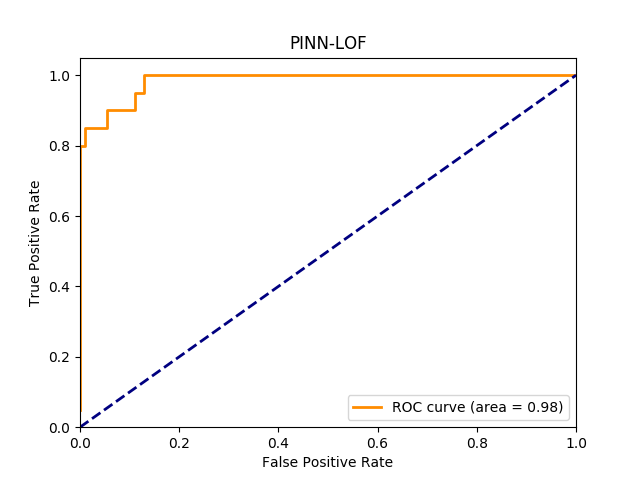
\includegraphics[width=65mm,height=40mm]{imagenes/pinn-lof-sintetic-roc.png} \\
    Score & Curca ROC para datos sinteticos \\[6pt]
    \multicolumn{2}{c}{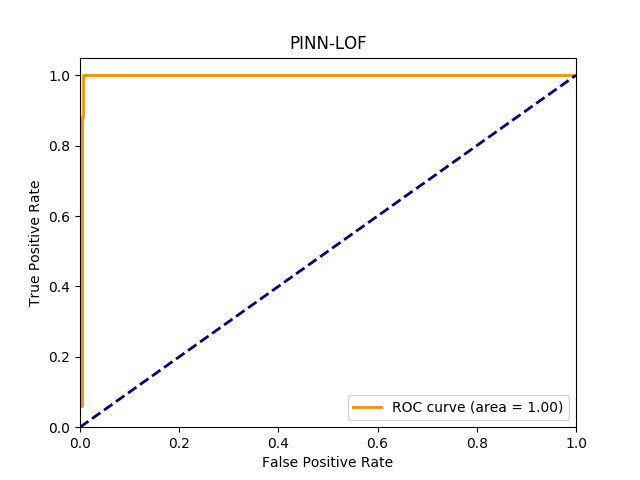
\includegraphics[width=65mm,height=39mm]{imagenes/pinn-lof-test.png} }\\
    \multicolumn{2}{c}{Curva ROC para datos reales}\\
    \end{tabular}
    \caption{\label{fig:pinnloftest} PINN-LOF test}
\end{figure}


\begin{figure}[H]
    \begin{tabular}{cc}
      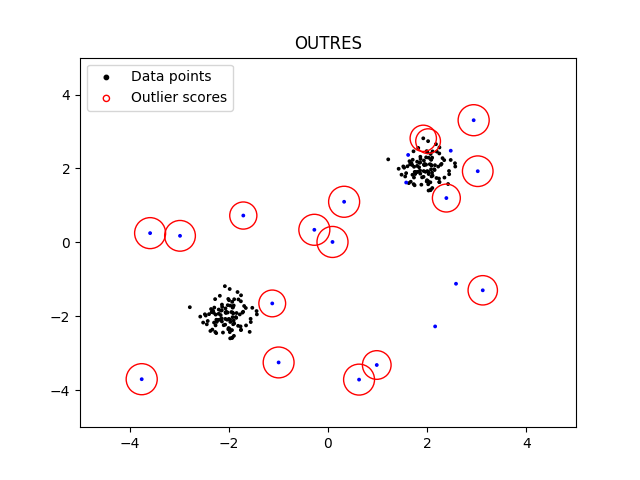
\includegraphics[width=65mm,height=40mm]{imagenes/outres-sintetico.png} &   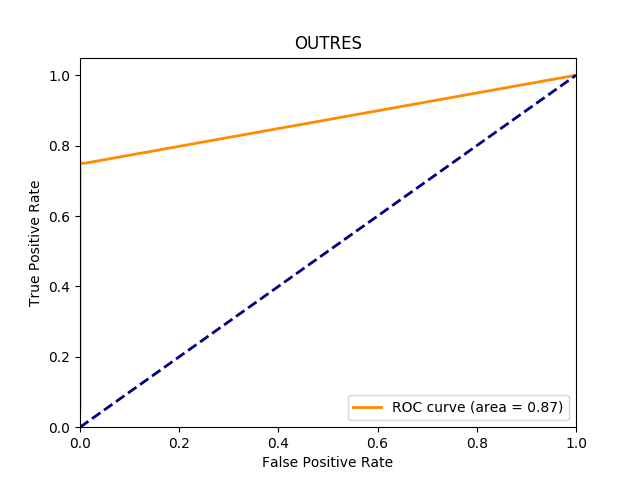
\includegraphics[width=65mm,height=40mm]{imagenes/outres-sintetic-roc.png} \\
    Score & Curca ROC para datos sinteticos \\[6pt]
    \multicolumn{2}{c}{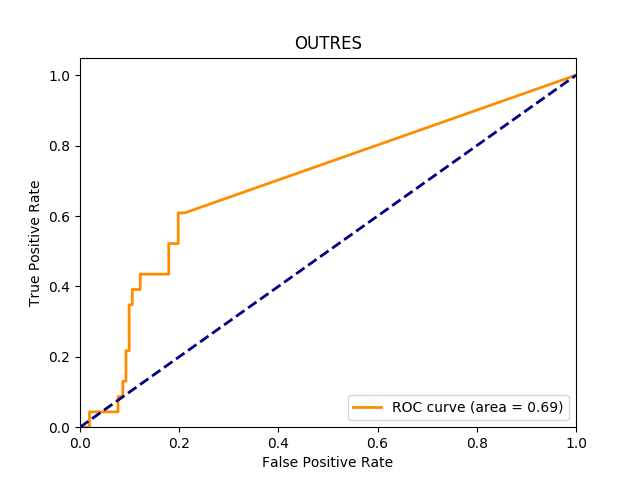
\includegraphics[width=65mm,height=39mm]{imagenes/outres-test.png} }\\
    \multicolumn{2}{c}{Curva ROC para datos reales}\\
    \end{tabular}
    \caption{\label{fig:outrestest} OUTRES test}
\end{figure}

\begin{figure}[H]
  \begin{tabular}{cc}
    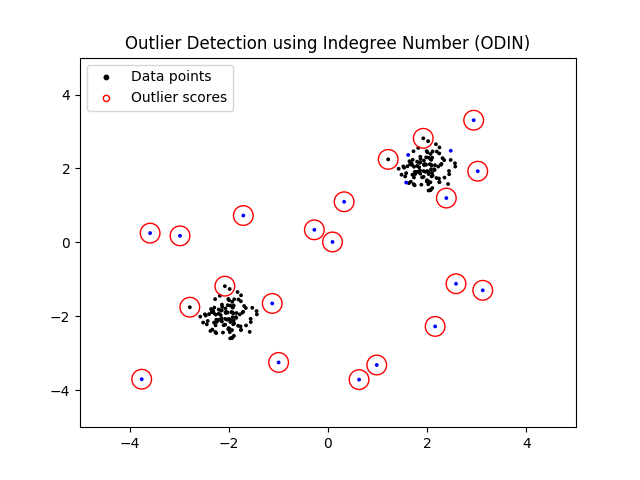
\includegraphics[width=65mm,height=40mm]{imagenes/odin-sintetico.png} &   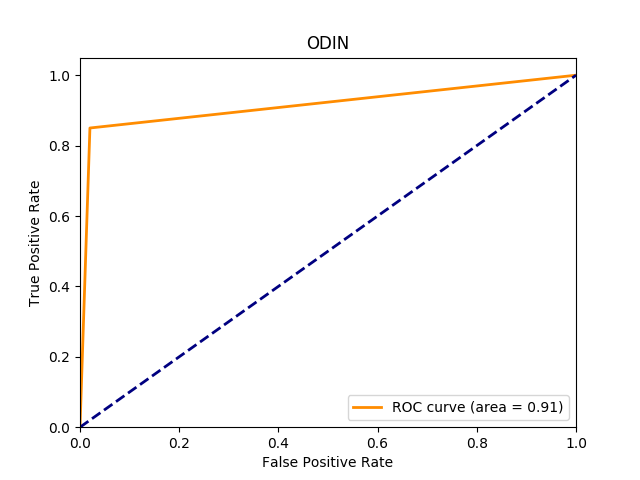
\includegraphics[width=65mm,height=40mm]{imagenes/odin-sintetic-roc.png} \\
  Score & Curca ROC para datos sinteticos \\[6pt]
  \multicolumn{2}{c}{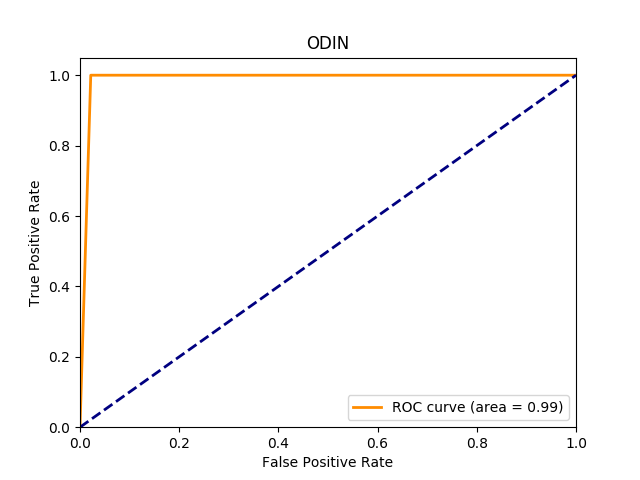
\includegraphics[width=65mm,height=39mm]{imagenes/odin-test.png} }\\
  \multicolumn{2}{c}{Curva ROC para datos reales}\\
  \end{tabular}
  \caption{\label{fig:odintest} ODIN test}
\end{figure}


\begin{figure}[H]
  \begin{tabular}{cc}
    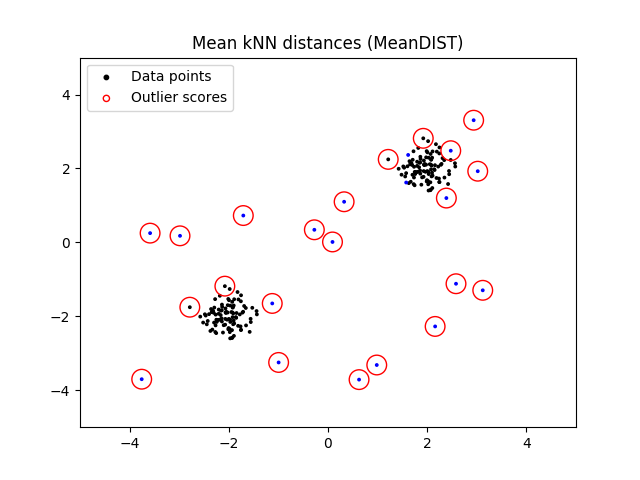
\includegraphics[width=65mm,height=40mm]{imagenes/meandist-sintetico.png} &   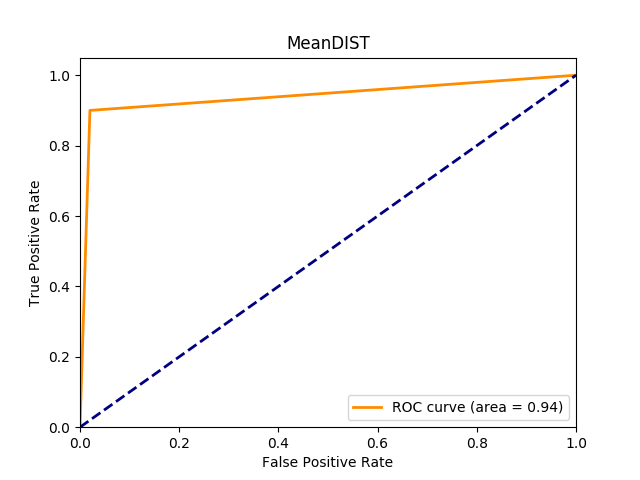
\includegraphics[width=65mm,height=40mm]{imagenes/meandist-sintetic-roc.png} \\
  Score & Curca ROC para datos sinteticos \\[6pt]
  \multicolumn{2}{c}{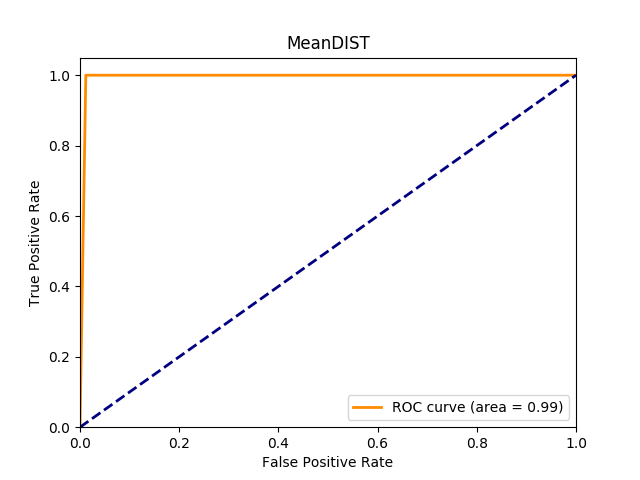
\includegraphics[width=65mm,height=39mm]{imagenes/meandist-test.png} }\\
  \multicolumn{2}{c}{Curva ROC para datos reales}\\
  \end{tabular}
  \caption{\label{fig:meandisttest} MeanDIST test}
\end{figure}

\begin{figure}[H]
  \begin{tabular}{cc}
    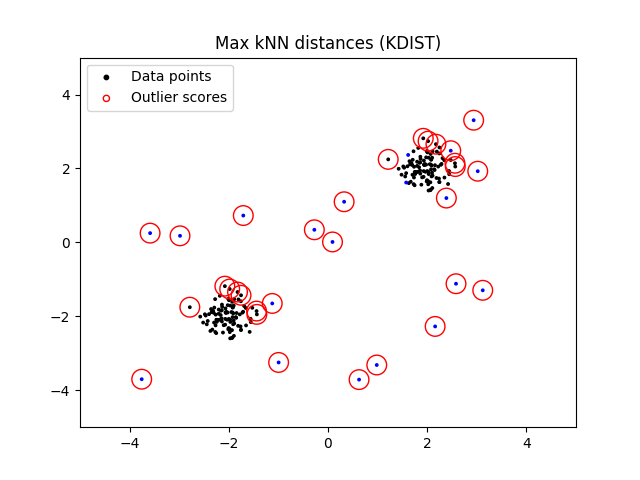
\includegraphics[width=65mm,height=40mm]{imagenes/kdist-sintetico.png} &   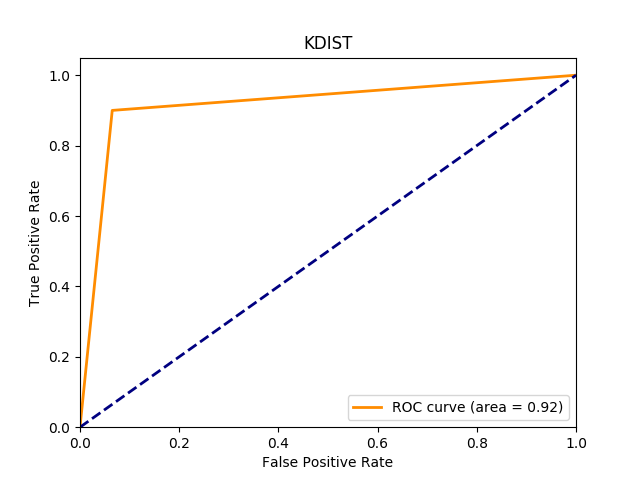
\includegraphics[width=65mm,height=40mm]{imagenes/kdist-sintetic-roc.png} \\
  Score & Curca ROC para datos sinteticos \\[6pt]
  \multicolumn{2}{c}{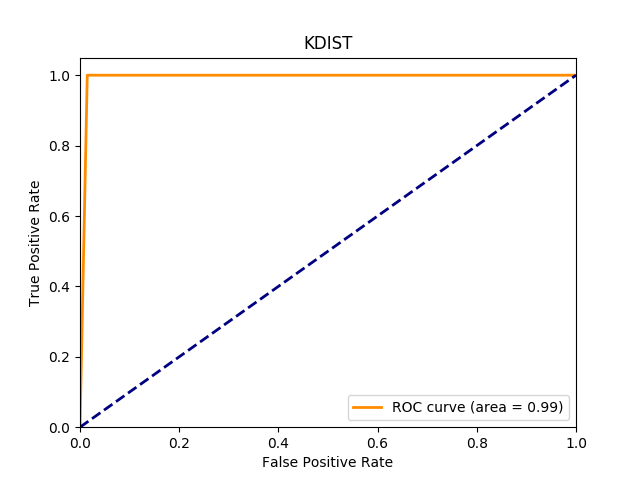
\includegraphics[width=65mm,height=39mm]{imagenes/kdist-test.png} }\\
  \multicolumn{2}{c}{Curva ROC para datos reales}\\
  \end{tabular}
  \caption{\label{fig:kdisttest} kDIST test}
\end{figure}

Como podemos tanto en los datos sintéticos como en el conjunto de datos reales
que hemos utilizado para probar nuestros algoritmos, los resultados son
muy buenos. Todos como podemos ver detectan casi todas las anomalías 
dándole una puntuación alta. Esto lo podemos ver en la primera figura 
donde el radio de los puntos azules, que son las anomalías, son mucho más
amplios que el resto de puntos concentrados en dos grupos.

Para reafirmar la idea tenemos la curva ROC y el área baja la curva que
determina la métrica AUC. Como podemos ver en la mayoría de casos La métrica nos 
indica que los resultados son muy buenos y que tenemos unos buenos métodos para afrontar
el problema.

Quizás podríamos pensar que esto son buenos resultados ya que usamos datos 
sintéticos. Para ello hemos cogido un conjunto de datos aleatorio del repositorio del
que disponíamos para experimentar que comentaremos más adelante. El conjunto de
datos se llama \textit{shuttle-c0-vs-c4.dat} y está compuesto por 9 variables enteras.
De este modo también probamos su correcto funcionamiento en casos más complejos.
Los resultados de dichas pruebas los tenemos en la tercera figura correspondiente a cada
algoritmo. Como podemos ver los resultados obtenidos en los datos sintéticos se mantienen,
y seguimos teniendo unos resultados fantásticos.

La sorpresa llegó con el mal desempeño de \textbf{OUTRES}. En primer lugar
tenemos que comentar que a pesar de conocer el hecho de su alta complejidad lo que podía
suponer un alto coste en tiempo, confiábamos en que la técnica de poda hiciera este algoritmo
útil ya que el procedimiento y técnica tenían una idea buena. En la práctica esta idea 
para la cual se realiza la poda, no tiene una buena utilidad. Esto se debe a que en datos 
reales la poda es difícil de realizar ya que es fácil que el test estadístico falle. A pesar de
subir el umbral intentado subir la poda sigue siendo costoso y se aumenta demasiado la poda, los
resultados empeoran. Por tanto, el algoritmo no solo es costoso en tiempo, sino que, además
es complicado conseguir un buen ajuste de los parámetros. Pero en realidad, los
resultados no son competitivos con el resto de algoritmos en este tipo de casos. A pesar de las pruebas
decidimos mantener este algoritmo ya que, aunque en nuestros conjuntos de datos no tenía los mejores factores 
para favorecer su mejor desarrollo, puede que a los usuarios futuros que utilicen
esta herramienta, le ayude y sea un algoritmo que, si se cumplen determinadas condiciones, su comportamiento
sea mejor incluso que los del resto. Este mejor comportamiento lo plantean los autores en 
\cite{mullerAdaptiveOutliernessSubspace2010}. 


En definitiva, podemos ver como nuestra biblioteca
puede afrontar y resolver el problema de la detección de anomalías
desde el enfoque de técnicas basadas en la proximidad. En cuanto a la implementación
de los algoritmos seleccionados queda demostrado que es correcta y robusta.




\section{Estudio experimental para problemas con alto desequilibrio}
En este punto del trabajo ya disponemos de la funcionalidad de nuestra biblioteca por lo que 
una vez que hemos ejemplificado el uso de los algoritmos, realizamos una experimentación 
para probar el comportamiento de nuestros algoritmos frente a 
una gran batería de conjuntos de datos. Con ello obtendremos una gran información y demostraremos 
el desempeño y la robustez de nuestro proyecto. Para ello hemos seleccionado conjuntos de clasificación 
binaria muy desbalanceada con ratios mayores que 9. En los problemas desbalanceados
lo que tenemos es una clase con un número muy pequeño de instancias con respecto
a la clase mayoritaria. El ratio es la relación entre el número de datos de una clase y
la minoritaria. Usamos este tipo de problemas porque, a diferencia de entornos puramente no
supervisados, en este caso disponemos de las etiquetas que usaremos, no para entrenar sino 
para medir el desempeño de los algoritmos. Además, tomamos este tipo de conjuntos de datos 
muy desbalanceados porque esperamos que las anomalías representen un porcentaje pequeño del 
número total de instancias.


Por tanto, la clase minoritaria se tomará como 
anomalías y la clase mayoritaria serán los casos normales de funcionamiento. 
Para medir el desempeño de cada algoritmo usaremos como en el apartado anterior la 
métrica \textbf{AUC} la cual nos ofrece una buena medida sobre el funcionamiento  
de nuestra biblioteca frente a los diversos problemas. 

Para cada algoritmo y cada conjunto de datos se ha realizado una búsqueda de los mejores
parámetros para buscar una puntuación adecuada. En el caso de \textbf{OUTRES}  y la 
complejidad hace inaccesible su uso para conjuntos de datos reales, por lo que no se 
han podido obtener resultados con este algoritmo. Los tiempos de ejecución son realmente
elevados por lo que realizar una busqueda de hiperparámetros y conseguir resultados se
convierte en algo inviable.



Como comentábamos en la introducción existe una biblioteca llamada \textbf{PyOD} 
\cite{zhaoPyODPythonToolbox2019} \cite{zhaoPythonToolboxScalable2019} 
que también implementa algunos algoritmos basados en proximidad, nuestra intención es usar el 
algoritmo \textbf{LOCI} \cite{papadimitriouLOCIFastOutlier2003} de dicha biblioteca  
para comparar los resultados con los nuestros y ver si nuestra biblioteca es competitiva.
Cabe destacar que la execución de \textbf{LOCI}, superaba con diferencia el tiempo de ejecución
de nuestros algoritmos. Para aclarar este punto exponemos nuestra experiencia en la 
experimentación. Si se ejecutaban todos los algoritmos, excepto \textbf{LOCI}, el tiempo de ejecución
era de 20 minutos. En caso de calcular los resultados de \textbf{LOCI}, fueron necesarios más de 2
días.
Esto confirma la idea de que nuestra biblioteca es competitiva en lo que se refiere a velocidad
y tiempo de computación.


Se han seleccionado 20 conjuntos de datos de la base de datos KEEL \cite{alcala-fdezKEELSoftwareTool2009} 
de donde hemos seleccionado un paquete de clasificación binaria muy desbalanceada. La ratio de  
desbalanceo en todos los casos es mayor que 9 y en algunos casos llega a más de 30. Por tanto, 
lo que hemos hecho ha sido tomar como anomalías la clase menos numerosa y el resto de ejemplos 
serán la clase normal. Con esta batería de conjuntos de datos será con la que experimentemos. 

Vamos a ver los resultados obtenidos en la siguiente tabla y los comentaremos posteriormente:

\begin{figure}[h]
  \center{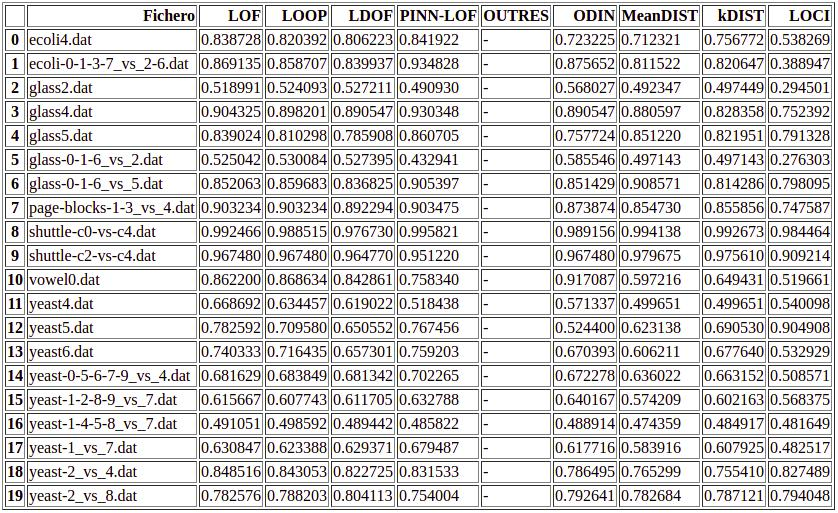
\includegraphics[width=\textwidth]
  {imagenes/resultados.jpeg}}
  \caption{\label{fig:resultados} Valores AUC de la experimentación}
\end{figure}

Como podemos ver en general los resultados son muy variados y fuertemente dependientes del conjunto
de datos al que se enfrenta. Vamos a comentar ciertas cosas que consideramos ciertamente 
interesantes.

En primer lugar, podemos ver como los resultados entre los 7 algoritmos de nuestra biblioteca
 son similares en cada conjunto de 
datos. En primer lugar tenemos que mencionar que en general \textbf{LDOF} no consigue mejores  
resultados que el resto de algoritmos en ningún conjunto de datos. A pesar de ello tampoco podemos 
considerar que obtenga resultados malos ya que está cerca del resto. Esto se debe a que  
\textbf{LDOF} está enfocado a conjuntos de datos dispersos y en nuestro caso teníamos como 
experimentación datos que anteriormente eran considerados una clase, por lo que es fácil suponer 
que entre una parte de los datos considerados anomalías podrían estar agrupados. Esto ha perjudicado 
un poco a \textbf{LDOF}. 

En segundo lugar podemos destacar el comportamiento de \textbf{PINN-LOF}. Su comportamiento es muy positivo
ya que en muchos casos, podemos observar cómo se cumple la necesidad de explorar subespacios. 
Como comentábamos en las explicaciones los algoritmos usan la distancia entre todas las dimensiones, 
esto hace que la diferencia se homogenice cuando realmente la anomalía se diferencia en una o varias subdimensiones. 
Con \textbf{PINN-LOF} seleccionamos subespacios aleatoriamente y se analiza si puede determinarse si es anomalía. 
en casos como en \textbf{ecoli-0-1-3-7-vs2-6, glass4, glass-0-1-6-vs-5} podemos ver que la ganancia es considerable 
con el resto de algoritmos. En algunos casos la ganancia es de $0.1$. Esto se debe a que en esa búsqueda aleatoria 
a través de los distintos subespacios, el algoritmo encuentra un subespacio donde es más fácil 
diferenciar las anomalías. Como podemos ver este enfoque nos puede aportar una mejora considerable. 
También se confirma las sospechas de que a mayor dimensionalidad las diferencia entre distancias se pierde 
ya que en este caso tenemos unos de los conjuntos con más dimensiones del conjunto.
Además, permite una aplicación de \textbf{LOF} de forma más eficiente al no usar todas las dimensiones.
La parte negativa de este algoritmo la encontramos en ejemplos como \textbf{yeast4}. Donde encontramos 
un resultado peor comparado con otros algoritmos. Esto se debe a la búsqueda aleatoria lo que en este 
caso ha propiciado un peor resultado por la elección de subespacios no muy buenos. Debemos  
mencionar que en las pruebas realizadas hemos observado que es un algoritmo totalmente dependiente de  
la aleatoriedad ya que depende totalmente de las elecciones que realiza. Influye más la aleatoriedad 
que los parámetros y ha sido difícil encontrar los parámetros correctos. 

Ahora vamos a analizar los resultados en conjunto de \textbf{LOF y LOOP} ya que se basaban 
en conceptos similares. Como podemos ver esto se ha reflejado en resultados similares. No existe 
una diferencia clara entre ambos algoritmos y los resultados en casi todos los casos son similares. 
Cabe resaltar que de forma general \textbf{LOF} consigue siempre una pequeña mejora que en algunos 
casos. Si se hace notable en algunos conjuntos como en \textbf{yeast5}. Como comentábamos y explicábamos anteriormente  
son algoritmos basados en conceptos similares. La gran ventaja de \textbf{LOOP} es que nos ofrece 
como resultado una probabilidad, lo que facilita su interpretabilidad y la comparación con otros  
algoritmos. 

En cuanto al comportamiento de \textbf{ODIN} podemos decir que realiza un desempeño notable. en general 
obtiene resultados muy similares al resto de algoritmos y en casos como en el conjunto de datos de  
\textbf{vowel0} se consigue un resultado mejor. En definitiva, es un algoritmo con un muy buen 
desempeño. El único inconveniente que podemos poner a este algoritmo es la elección 
de hiperparámetros, ya que el parámetro clave es la selección del umbral del grado de vecinos 
recíprocos que permitimos. Esto hace que sea algo más complejo su ajuste porque para un buen ajuste sería necesario 
conocer información adicional del conjunto de datos o una aproximación del número de anomalías que esperamos 
encontrar. 

Analizamos el comportamiento de \textbf{MeanDIST y kDIST} conjuntamente ya que la idea que subyace bajo 
ambos algoritmos es la misma. En primer lugar, debemos mencionar que, aunque su desempeño de forma general 
suele ser más pobre que el resto de algoritmos, aunque muy cerca. También debemos mencionar que existen casos 
en los que se encuentran soluciones realmente destacables en comparación con el resto, como por ejemplo en  
el conjunto \textbf{glass-0-1-6-vs-5} donde se alcanza una puntuación de. Por tanto, son algoritmos 
que, a pesar de usar una idea más simple para detectar anomalías, existen casos en los que presentan una ventaja 
y no pueden ser descartados. Por otro lado, en este caso se reafirma la idea de que los algoritmos estan condicionados 
al conjunto de datos. Como podemos ver no podemos decir que sea mejor usar la media de distancias o la distancia mayor 
ya que existen casos para los cuales uno tiene un mejor desempeño que el otro. En estos algoritmos nos ha sorprendido 
como un enfoque tan sencillo puede conseguir resultados bastante buenos, aunque queda claro que si queremos 
ser más precisos y conseguir resultados mejores, son enfoques que pueden no ser suficientes. 

Por otro lado, nos sorprende el comportamiento de \textbf{OUTRES} 
ya que los conceptos en los que se basa son similares a \textbf{PINN-LOF}, 
la búsqueda de anomalías en subespacios. En \textbf{PINN-LOF} hemos visto como incluso usando 
una selección aleatoria esto puede generar muy buenos resultados y que realmente es necesaria esa  
búsqueda en subespacios, cuando la dimensión crece, no solo por eficiencia sino también por realizar 
una mejor aproximación. En el caso de \textbf{OUTRES} su parte positiva es a la vez la negativa. Considerábamos 
que era muy interesante al realizar esta búsqueda de subespacios relevantes y que podía generar grandes resultados. 
La realidad es que ese análisis tan exhaustivo lo convierte en un algoritmo con una complejidad inaplicable. 
Cierto es que se diseña un sistema de poda, pero en los ejemplos reales este sistema no consigue una poda necesaria 
para hacer eficiente el algoritmo. 

Por último, tenemos los resultados del algoritmo \textbf{LOCI} procedente de la biblioteca PyOD \cite{zhaoPyODPythonToolbox2019}.
Respecto a esta biblioteca ya comentábamos como nuestra biblioteca tenía un mejor desempeño en cuanto a tiempo de ejecución.
En cuanto a los resultados podemos observar la última columna y comparar con el resto de columnas. Claramente podemos ver que existe
una gran diferencia en la puntuación obtenida. Solo en el archivo \textbf{yeast5} consigue un resultado bastante mejor que el resto de
algoritmos. Como conclusión de esta experimentación podemos confirmar que nuestra biblioteca no es solo competitiva a nivel de tiempos
sino que ofrece unos resultados bastante mejores y que ofrece una solución al problema de la detección de anomalías de calidad.

Como aclaración podemos ver que hay conjuntos de datos en los que ningún algoritmo consigue buenos resultados, por ello 
podemos considerar que esto se debe a los datos subyacentes y que realmente sea complicado una separación entre 
anomalías y datos normales. 

Como conclusión final de esta experimentación podemos decir que por un lado tenemos a \textbf{LOF y LOOP}, 
dos algoritmos con muy buenos resultados y sobre todo estables. Consiguen un rendimiento bueno  
en todos los conjuntos aunque destacar que \textbf{LOF} obtiene un mejor desempeño y \textbf{LOOP} nos 
proporciona una interpretabilidad más fácil. Por otro lado hemos analizado el comportamiento de \textbf{LDOF} 
que en general también consigue buenos resultados, aunque no destaca ya que está diseñado para conjuntos de datos 
más dispersos. También tenemos \textbf{PINN-LOF} un algoritmo capaz de conseguir mejores resultados que el resto aunque 
muy inestable por su componente aleatoria. Por último tenemos \textbf{ODIN} el cual nos ofrece muy buenos resultados
pero tiene una mayor complejidad para ajustar los hiperparámetros y \textbf{MeanDIST y kDIST}, algoritmos más simples y 
fáciles de interpretar aunque con un desempeño bueno pero más pobre.



%
\chapter{Conclusiones} 

En este proyecto se ha implementado una biblioteca con 5 algoritmos 
de detección de anomalías basados en proximidad. Cada uno de ellos  
busca afrontar el problema y sus inconvenientes desde una perspectiva 
y técnica diferente. En el momento de esta publicación no existe  
ninguna biblioteca con todos estos algoritmos ya sea en Python o  
en otros lenguajes de programación. 
 

A nivel técnico, hemos visto como existen multitud de factores que  
pueden afectar al resultado final por lo que cada enfoque puede ser 
interesante según los datos a los que nos enfrentamos. También hemos 
visto como el problema de la detección de anomalías tiene una clara  
aplicación al mundo real y nuestros algoritmos pueden aplicarse a  
conjuntos de datos reales. 
 

En conclusión, hemos desarrollado una biblioteca o herramienta que cumple 
los requisitos que nos planeábamos al comienzo del estudio, buenos resultados 
con un pequeño tiempo de ejecución, estandarización, respuesta clara y seguridad.  
 
\section{Trabajo futuro} 
Como trabajos futuros se podrían seguir implementando más algoritmos 
para aumentar la paleta de posibilidades para aplicar ante los diferentes 
problemas que les pueden surgir a los usuarios finales de nuestra biblioteca. 

También podríamos ampliar el campo de técnicas incluidas e introducir  
algoritmos de otros enfoques como puede ser técnicas estadísticas, que  
aumentarían la utilidad y funcionalidad de nuestra biblioteca.




%
\chapter{Apéndice}
En este apartado se introduce la documentación de la biblioteca,
con la descripción de cada clase. El objetivo de dicha documentación es 
facilitar al usuario final el uso de la biblioteca, la cual puede 
consultar online, para tener una referencia y breve
descripción de los métodos.

Aquí se introduce la versión pdf de dicha documentación pero
podemos encontrar dicha documentación en línea en el repositorio
del proyecto en GitHub \cite{Miki97TFGOutlierDetectionHttps} y en el repositorio de 
PyPI \cite{PyDBODDistancesBased}


\setboolean{@twoside}{false}

\addcontentsline{toc}{chapter}{Manual PyDBOD}

\includepdf[scale= 1,pages=-, ]{documentation.pdf}
%
\includepdf[scale=0.8,pages=-,pagecommand=\subsection{blub}]{documentation}
%
%%\chapter{Conclusiones y Trabajos Futuros}
%
%
%%\nocite{*}
%\bibliography{bibliografia/bibliografia}\addcontentsline{toc}{chapter}{Bibliografía}
\bibliography{TFG-MiguelAngelRobles.bib}
\bibliographystyle{ieeetr}
%\bibliographystyle{miunsrturl}
%
%\appendix
%\input{apendices/manual_usuario/manual_usuario}
%%\input{apendices/paper/paper}
%\input{glosario/entradas_glosario}
% \addcontentsline{toc}{chapter}{Glosario}
% \printglossary
\chapter*{}
\thispagestyle{empty}

\end{document}
